% This is the Reed College LaTeX thesis template. Most of the work 
% for the document class was done by Sam Noble (SN), as well as this
% template. Later comments etc. by Ben Salzberg (BTS). Additional
% restructuring and APA support by Jess Youngberg (JY).
% Your comments and suggestions are more than welcome; please email
% them to cus@reed.edu
%
% See http://web.reed.edu/cis/help/latex.html for help. There are a 
% great bunch of help pages there, with notes on
% getting started, bibtex, etc. Go there and read it if you're not
% already familiar with LaTeX.
%
% Any line that starts with a percent symbol is a comment. 
% They won't show up in the document, and are useful for notes 
% to yourself and explaining commands. 
% Commenting also removes a line from the document; 
% very handy for troubleshooting problems. -BTS

% As far as I know, this follows the requirements laid out in 
% the 2002-2003 Senior Handbook. Ask a librarian to check the 
% document before binding. -SN

%%
%% Preamble
%%
% \documentclass{<something>} must begin each LaTeX document
\documentclass[12pt,twoside]{reedthesis}
% Packages are extensions to the basic LaTeX functions. Whatever you
% want to typeset, there is probably a package out there for it.
% Chemistry (chemtex), screenplays, you name it.
% Check out CTAN to see: http://www.ctan.org/
%%
\usepackage{graphicx,latexsym} 
\usepackage{amssymb,amsthm,amsmath}
\usepackage{longtable,booktabs,setspace} 
\usepackage{chemarr} %% Useful for one reaction arrow, useless if you're not a chem major
\usepackage[hyphens]{url}
\usepackage{subcaption}
\usepackage{rotating}
\usepackage{ifthen}
\usepackage{multirow}
\usepackage{color}
\usepackage[export]{adjustbox}[2011/08/13]
\graphicspath{{./Figs/}} % Set graphics path
% Comment out the natbib line above and uncomment the following two lines to use the new 
% biblatex-chicago style, for Chicago A. Also make some changes at the end where the 
% bibliography is included. 
%\usepackage{biblatex-chicago}
%\bibliography{thesis}

% \usepackage{times} % other fonts are available like times, bookman, charter, palatino


%%%% REFERENCES %%%%%
\newcommand{\rf}     [1] {~\cite{#1}}
\newcommand{\refref} [1] {ref.~\cite{#1}}
\newcommand{\refRef} [1] {Ref.~\cite{#1}}
\newcommand{\refrefs}[1] {refs.~\cite{#1}}
\newcommand{\refRefs}[1] {Refs.~\cite{#1}}
\newcommand{\refeq}  [1] {Eq.~(\ref{#1})}
\newcommand{\refeqs} [2]{Eqs.~\ref{#1} and \ref{#2}}
\newcommand{\refFig} [1] {Fig.~\ref{#1}}
\newcommand{\refFigs} [2] {Figs.~\ref{#1} and~\ref{#2}}
\newcommand{\reftab} [1] {Table~\ref{#1}}
\newcommand{\refTab} [1] {Table~\ref{#1}}
\newcommand{\reftabs}[2] {tables~\ref{#1} and~\ref{#2}}
\newcommand{\refsect}[1] {Section~\ref{#1}}
\newcommand{\refsects}[2] {Sections~\ref{#1} and \ref{#2}}
\newcommand{\refSect}[1] {Section~\ref{#1}}
\newcommand{\refSects}[2] {Sects.~\ref{#1} and \ref{#2}}
\newcommand{\refsecttosect}[2] {Sects.~\ref{#1} to~\ref{#2}}
\newcommand{\refappe}[1] {appendix~\ref{#1}}
\newcommand{\refappes}[2] {appendices~\ref{#1} and~\ref{#2}}
\newcommand{\refAppe}[1] {Appendix~\ref{#1}}
\newcommand{\refChapter}[1]{Chapter~\ref{#1}}
\newcommand{\refChapt}[1]{Chapt.~\ref{#1}}
\newcommand{\ignore}[1]{}
\newcommand{\nobibentry}[1]{{\let\nocite\ignore\bibentry{#1}}}
\newcommand{\bibfnamefont}[1]{#1}
\newcommand{\bibnamefont}[1]{#1}


%%%% SYMBOLS %%%%
\newcommand{\ReN}{\ensuremath{Re}} % Reynolds number

%%%% ABBREVIATIONS %%%%%
\newcommand{\etc}{{etc.}}       % APS
\newcommand{\etal}{{\em et al.}}    % etal in italics, APS too
\newcommand{\ie}{{i.e.}}        % APS
\newcommand{\cf}{{\em cf.\ }}     % APS
\newcommand{\eg}{{e.g.\ }}        % APS, OUP, hard space '\eg\ NextWord'

%%%%% EDITING COMMANDS %%%%%
\newcommand{\DB}[2]{$\footnotemark\footnotetext{DB #1: {\color{red}#2}}$} %date, comment
\newcommand{\DBedit}[1]{{\color{red}#1}}
\newcommand{\MC}[2]{$\footnotemark\footnotetext{DB #1: {\color{green}#2}}$} %date, comment
\newcommand{\MCedit}[1]{{\color{green}#1}}
 % Load thesis specific macros

\title{On Bouncing Oil Drops}
\author{Miguel B. Conner}
\date{May 2015}
\division{Mathematics and Natural Sciences}
\advisor{Daniel Borrero}
\department{Physics}

\setlength{\parskip}{0pt}
%%
%% End Preamble
%%
%% The fun begins:
\begin{document}

  \maketitle
  \frontmatter % this stuff will be roman-numbered
  \pagestyle{empty} % this removes page numbers from the frontmatter

% Acknowledgements (Acceptable American spelling) are optional
% So are Acknowledgments (proper English spelling)
	% Acknowledgements (Acceptable American spelling) are optional
% So are Acknowledgments (proper English spelling)
    \chapter*{Acknowledgements}
	I want to thank a few people.
	
	%Help with thesis
	%Daniel, Jay, Bob. Kai, Lily, jack for reading drafts. daniel
	
	%Physics profs
	%Daniel, Darrell, Nelia, johnny, Joel, Lucas
	
	%Other profs
	% Albert, Libby, Alan (sp?), 
	
	% Parents
	
	% Kai
	
	% Lily and Clops
	
	

% The preface is optional
% To remove it, comment it out or delete it.
%	% The preface is optional
% To remove it, comment it out or delete it.
    \chapter*{Preface}
	This is an example of a thesis setup to use the reed thesis document class.

  \tableofcontents
% if you want a list of tables, optional
%  \listoftables
% if you want a list of figures, also optional
%  \listoffigures
		
% The abstract is not required if you're writing a creative thesis (but aren't they all?)
% If your abstract is longer than a page, there may be a formatting issue.
	% The abstract is not required if you're writing a creative thesis (but aren't they all?)
% If your abstract is longer than a page, there may be a formatting issue.
    \chapter*{Abstract}
	In 2005 Yves Couder's group discovered that and oil droplet placed on a vibrating bath of the same oil would bounce along the surface of the oil indefinitely, propelled by the waves it created \rf{Couder2005a}. This ``walker" exhibits many behaviors analogous to those observed in quantum systems, such as single particle double slit diffraction \rf{double-slit}, quantized orbits \rf{Oza2014}, and among others \rf{pilot-wave}, tunneling \rf{tunneling}. Tunneling occurs when a droplet interacts with a subsurface barrier; the droplet either passes over or reflects off of the barrier. In experiments described here, we studied the dependence of the tunneling probability on the height of a barrier of width $e=3.0~\mathrm{mm}$. It was determined that tunneling occurred for depths $h>1.0~\mathrm{mm}$, and appeared probabilistic at an oil depth of $h=1.25~\mathrm{mm}$. It was also observed that droplets with higher momentum are more likely to tunnel. 
%		\chapter*{Dedication}
	You can have a dedication here if you wish.

  \mainmatter % here the regular arabic numbering starts
  \pagestyle{fancyplain} % turns page numbering back on

% Double spacing: if you want to double space, or one and a half 
% space, uncomment one of the following lines. You can go back to 
% single spacing with the \singlespacing command.
% \onehalfspacing
% \doublespacing

	%%The \introduction command is provided as a convenience.
%if you want special chapter formatting, you'll probably want to avoid using it altogether
		
\chapter*{Introduction}
    \addcontentsline{toc}{chapter}{Introduction}
		\chaptermark{Introduction}
		\markboth{Introduction}{Introduction}
% The three lines above are to make sure that the headers are right, that the intro gets included in the table of contents, and that it doesn't get numbered 1 so that chapter one is 1.





	(Important: Particle-wave association on a fluid interface (Protiere 2006)).
	    
	    In 2005, Yves Couder showed that bouncing oil drops on vertically vibrating fluid bath exhibited properties analogous to the paradoxical properties seen only at the quantum scale (CITE: Dynamical phenomena:  Walking and orbiting droplets?). Couder, John Bush, and others have shown that this system can reproduce double-slit single-particle interference, orbiting, tunneling, quantized orbits, spin, and more.

	    	    \subsection{Faraday Waves}
	    
	    
	?

	    
	    \subsection{Bouncing Droplets}
	    Though it had been seen for at least a century, the phenomena of droplets bouncing on a fluid bath was first explained by Jearl Walker in 1978\rf{Walker}. The investigations began with a simple droplet of water falling onto a bath of water, and remaining just a second too long before coalescence.\footnote{I don't drink coffee so I haven't seen this, but everyone seems to cite that this occurrs with coffeemakers, as the coffee drips into the pot.} It was then discovered that adding detergent to the water and then vibrating the bath would extend the lifetime of these droplets from fractions of a second to several minutes. Because these droplets are bouncing at frequencies of around 50 Hz (50 bounces per second) and the droplets are very small to begin with (with a diameter of a millimeter or less), it can be difficult to observe even the main mechanisms that drive the behaviour. A key insight by Walker was to flash a strobelight at a frequency slightly slower than the rate of vibration of the fluid bath, that way he could observe the droplet bouncing as if in slow motion.
	    
	    Walker found that a trapped film of air kept the droplet and the bath from touching, as shown in \refFig{bounce}. That is, the droplet is bouncing on a layer of air that's struggling to get out of the way but because the bounce happens so quickly, the fluid droplet and the fluid bath never touch. Walker concluded that the leakage rate of this trapped pocket of air depends on three factors: the nature of surface tension of the fluid bath, the viscosity of the droplet and the fluid bath, and the viscocity of the air. The bath must be of uniform surface tension and free from particulate matter floating atop the bath, since both will lead to coalescence. Higher viscosity fluids translate to longer droplet lifetimes, since more viscous fluids keep air from escaping the pocket. Finally, adjusting the frequency and the amplitudes of the vibrations also affects droplet lifetime.\footnote{Reedie Andrew Case ('92) wrote his thesis ``Oil on Troubled Water: The Extension of Floating Drop Lifetimes Due to Interface Vibration" where he looked at droplet lifetime by the frequency of vibration.}   
	     
	    More recent research suggests that a droplet fluid like silicone oil could bounce indefinately of a vibrating bath\rf{Couder2005a}. The long lifetime occurs not only because silicone oil has a high viscosity, but also because it has a \textit{low} surface tension. A low surface tension is beneficial because it makes the oil bath relatively immune to surfactants (surface acting agents) or contaminations which would otherwise make the surface tension nonuniform, and thus create a coalescence event. 
	    
	    
	    
	    	    
	   	        
	    %(NONCOALESCENCE AND NONWETTING BEHAVIOR OF LIQUIDS
%Annual Review of Fluid Mechanics
%Vol. 34: 267-289 (Volume publication date January 2002)
%DOI: 10.1146/annurev.fluid.34.082701.154240
%G. Paul Neitzel1 and Pasquale Dell'Aversana2
%)

	    
	 
	    
	    	    \subsection{Walking Droplets}
	    
	       It was Couder who then showed that an oil droplet could live for much longer. Long lifetimes meant that the focus could shift from how the doplet bounced (short time scale) to its interactions with other droplets and its motion (longer time scale).
	       
	       Every time the droplet impacts the bath, it creates a radial traveling wave. If the bouncing droplet impacts the wavefield in such a way that it recives a lateral force from the slope of the wave, then it will be pushed to the side slightly. The next time the droplet makes contanct with the bath, it will again make contact with a slope, and be pushed to the side. This propels the bouncing droplet, causing it to ``walk" across the surface of the bath. These ``walkers" turned out to have particularly interesting behaviours. Indeed, in 2006 Yves Couder and Emmanuel Fort showed that these droplets mimicked the behavior of electrons in the hallmark experiment of quantum weirdness: the double slit experiment. This was the first time that microscopic scale behavior had ever been seen at a macroscopic level, and it sparked interest in the experiment.
	    
	    
	
	%\chapter*{Blog}
        \addcontentsline{toc}{chapter}{Blog}
        \chaptermark{Blog}
	\markboth{Blog}{Blog}
	
	This is the portion of the thesis that I will update regularly with rough notes, lit reviews, results, etc. some of which will be worked in to the real document after some polishing. 

	
	
	\section{To Do}
	\begin{itemize}
	\item{Analyze data. Miguel 4/6/15}
	\item{Write Intro, Ch 1, Ch 3, and Conclusion. Miguel 4/6/15}
     \item{Learn de Broglie's interpretation of QM. Miguel 11/6/14}
	\end{itemize}
	
	\subsection{Done}
	\begin{itemize}
	 \item{Take data. Miguel 12/2/14}
        \item{Figure out citations. 4/6/15}
	 \item{Set up Accelerometer (Finally--ugh). Miguel 
 2/20/15}
     \item{Get New Silicone Oil. Miguel 1/10/15}
     \item{Send copy of Lit Rev to Daniel to proofread. 12/23/14}
	\item{Find walking regime. Miguel 11/20/14}
	\item{Order Accelerometer. Miguel 11/6/14}
	\item{Learn Basics of Bohmian Mechanics. Miguel 10/28/14}
	\item{Make tray. Miguel 10/20/14}
	\item{Sort out camera situation. Miguel 10/20/14}
	\item{Obtain flashdrives.    Miguel 9/30/14}
	\item{Learn how to use the new \LaTeX\ and Github setup. Miguel 9/30/14}
	\end{itemize}
	
	\section{Literature Review}
	
(Important: Particle-wave association on a fluid interface (Protiere 2006)).
	    
	    In 2005, Yves Couder showed that bouncing oil drops on vertically vibrating fluid bath exhibited properties analogous to the paradoxical properties seen only at the quantum scale (CITE: Dynamical phenomena:  Walking and orbiting droplets?). Couder, John Bush, and others have shown that this system can reproduce double-slit single-particle interference, orbiting, tunneling, quantized orbits, spin, and more. The trajectory of the droplet can be modeled mathematically, and the dynamics of the walker have similarities to de Broglie's theory of quantum mechanics (CITE: Bush 2015).
	    
	    The literature review will begin with a description of Faraday waves and the basic dynamics of a bouncing droplet and a walking droplet. Then we will describe in detail a few of the important quantum-like properites of this system. 
	    
	    	    \subsection{Faraday Waves}
	    
	    
	?

	    
	    \subsection{Bouncing Droplets}
	    Though it had been around for at least a century, the phenomena of droplets bouncing on a vibrating fluid bath was first explained by Jearl Walker in 1978 CITE: WALKER. The first experiments looked at water droplets (bouncing on a vibrating water bath) that persisted for several seconds. Adding detergent to the water and modifying the frequency of vibration increased droplet's lifetime to minutes. Conversely any particulate impurities descrease the droplet's lifetime. Walker concluded that the droplets failed to coalesce because a layer of air trapped between the droplet and the bath would keep the two separate.\footnote{Reedie ??? wrote his thesis titled: ``???" on this very topic! } In other words, the droplet bounces on a cushion of air.
	        
	    %(NONCOALESCENCE AND NONWETTING BEHAVIOR OF LIQUIDS
%Annual Review of Fluid Mechanics
%Vol. 34: 267-289 (Volume publication date January 2002)
%DOI: 10.1146/annurev.fluid.34.082701.154240
%G. Paul Neitzel1 and Pasquale Dell'Aversana2
%)

	    
	 
	    
	    	    \subsection{Walking Droplets}
	    
	       It was Couder who then showed that an oil droplet could live for much longer. Long lifetimes meant that the focus could shift from how the doplet bounced (short time scale) to its interactions with other droplets and its motion (longer time scale).
	       
	       Every time the droplet impacts the bath, it creates a radial traveling wave. If the bouncing droplet impacts the wavefield in such a way that it recives a lateral force from the slope of the wave, then it will be pushed to the side slightly. The next time the droplet makes contanct with the bath, it will again make contact with a slope, and be pushed to the side. This propels the bouncing droplet, causing it to ``walk" across the surface of the bath. These ``walkers" turned out to have particularly interesting behaviours. Indeed, in 2006 Yves Couder and Emmanuel Fort showed that these droplets mimicked the behavior of electrons in the hallmark experiment of quantum weirdness: the double slit experiment. This was the first time that microscopic scale behavior had ever been seen at a macroscopic level, and it sparked interest in the experiment.
	    
	    
	    \subsection{Macroscopic Quantum Scale Behaviors} 
	    \subsubsection{Basic Parameters}
	       Consider a fluid of density $\rho$, viscosity $\nu$, and surface tension $\sigma$, in a bath of depth $H$ driven vertically at an amplitude $A_0$ at frequency $f=\omega/{2\pi}$. By defining $\mathnormal{\gamma}=A_0\omega^2$, the effective gravity in the frame of reference of the bath is $g+\gamma~\mathrm{sin}(\omega t)$. 
	       
	   \begin{figure}[h]
	       \centering
	    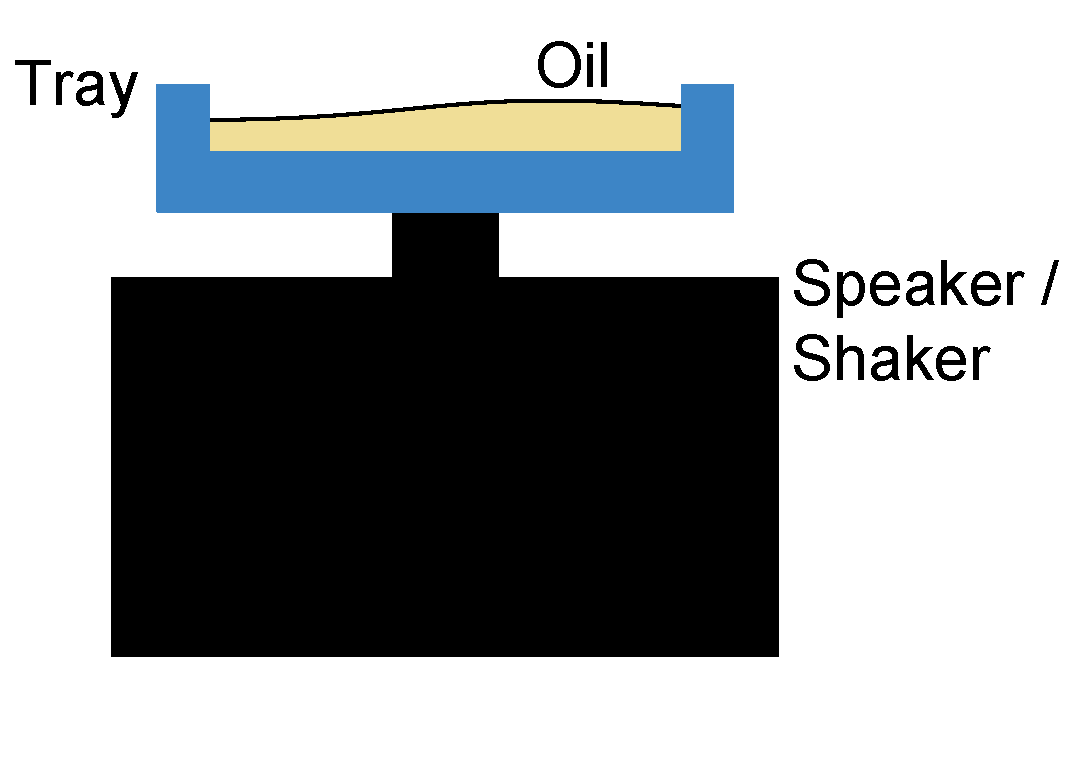
\includegraphics[scale=0.35]{HQASetup.pdf}
	     \caption{The experimental setup. The tray vibrates with an amplitude $A_0$.}
	 \label{regime}
	\end{figure}
	       
	       The oil droplet of diameter $D$ bounces in the regime $\gamma<\gamma_F$, where $\gamma_F$ is the Faraday threshold (at this point, Fraday waves appear). The important experimental limits are outlined in \refTab{approxlimits}. 
	       \begin{table}[htdp] 
\caption[Basic Table 1]{Approximate Limits for Bouncing Drop Behavior} 
\begin{center} 
\begin{tabular}{c c c} 
\toprule 
  Parameter &  Lower Limit & Upper Limit \\
  \midrule
Viscocity $\nu$ (cSt) & 10 & 100 \\ 
Bath Depth $H$ (mm) & 4 & 10 \\
Frequency $f$ (Hz) & 20 & 150 \\
Amplitude $A_0$ (mm) & 0.1 & 1 \\
Drop Diameter $D$ (mm) & 0.6 & 1.0 \\
\bottomrule 
\end{tabular}
\end{center}
\label{approxlimits} 
\end{table}	

For certain parameters, the bouncing drop will behave differently. The vibration number describes ``the relative magnitude of the forcing frequency and the drop's natural oscillation frequency," and is given by:
	       	      
\begin{equation} \label{vibrationnumber}
V_i = \frac{\omega}{2}\sqrt{\frac{\rho D^3}{2\sigma}}
\end{equation}   	       	       
	       	       The natural frequency of the droplet occurs around $V_i = 0.65$, where the droplet can exhibit both walking and bouncing behaviors. Setting up a plot with $V_i$ on the y axis and (dimensionless) ${\gamma}/{g}$ on the x axis can help in showing the behavior of the droplet, shown in \refFig{regime}. 
	    
	    \begin{figure}[h]
	% the options are h = here, t = top, b = bottom, p = page of figures.
	% you can add an exclamation mark to make it try harder, and multiple
	% options if you have an order of preference, e.g.
	% \begin{figure}[h!tbp]
	   
	       \centering
	    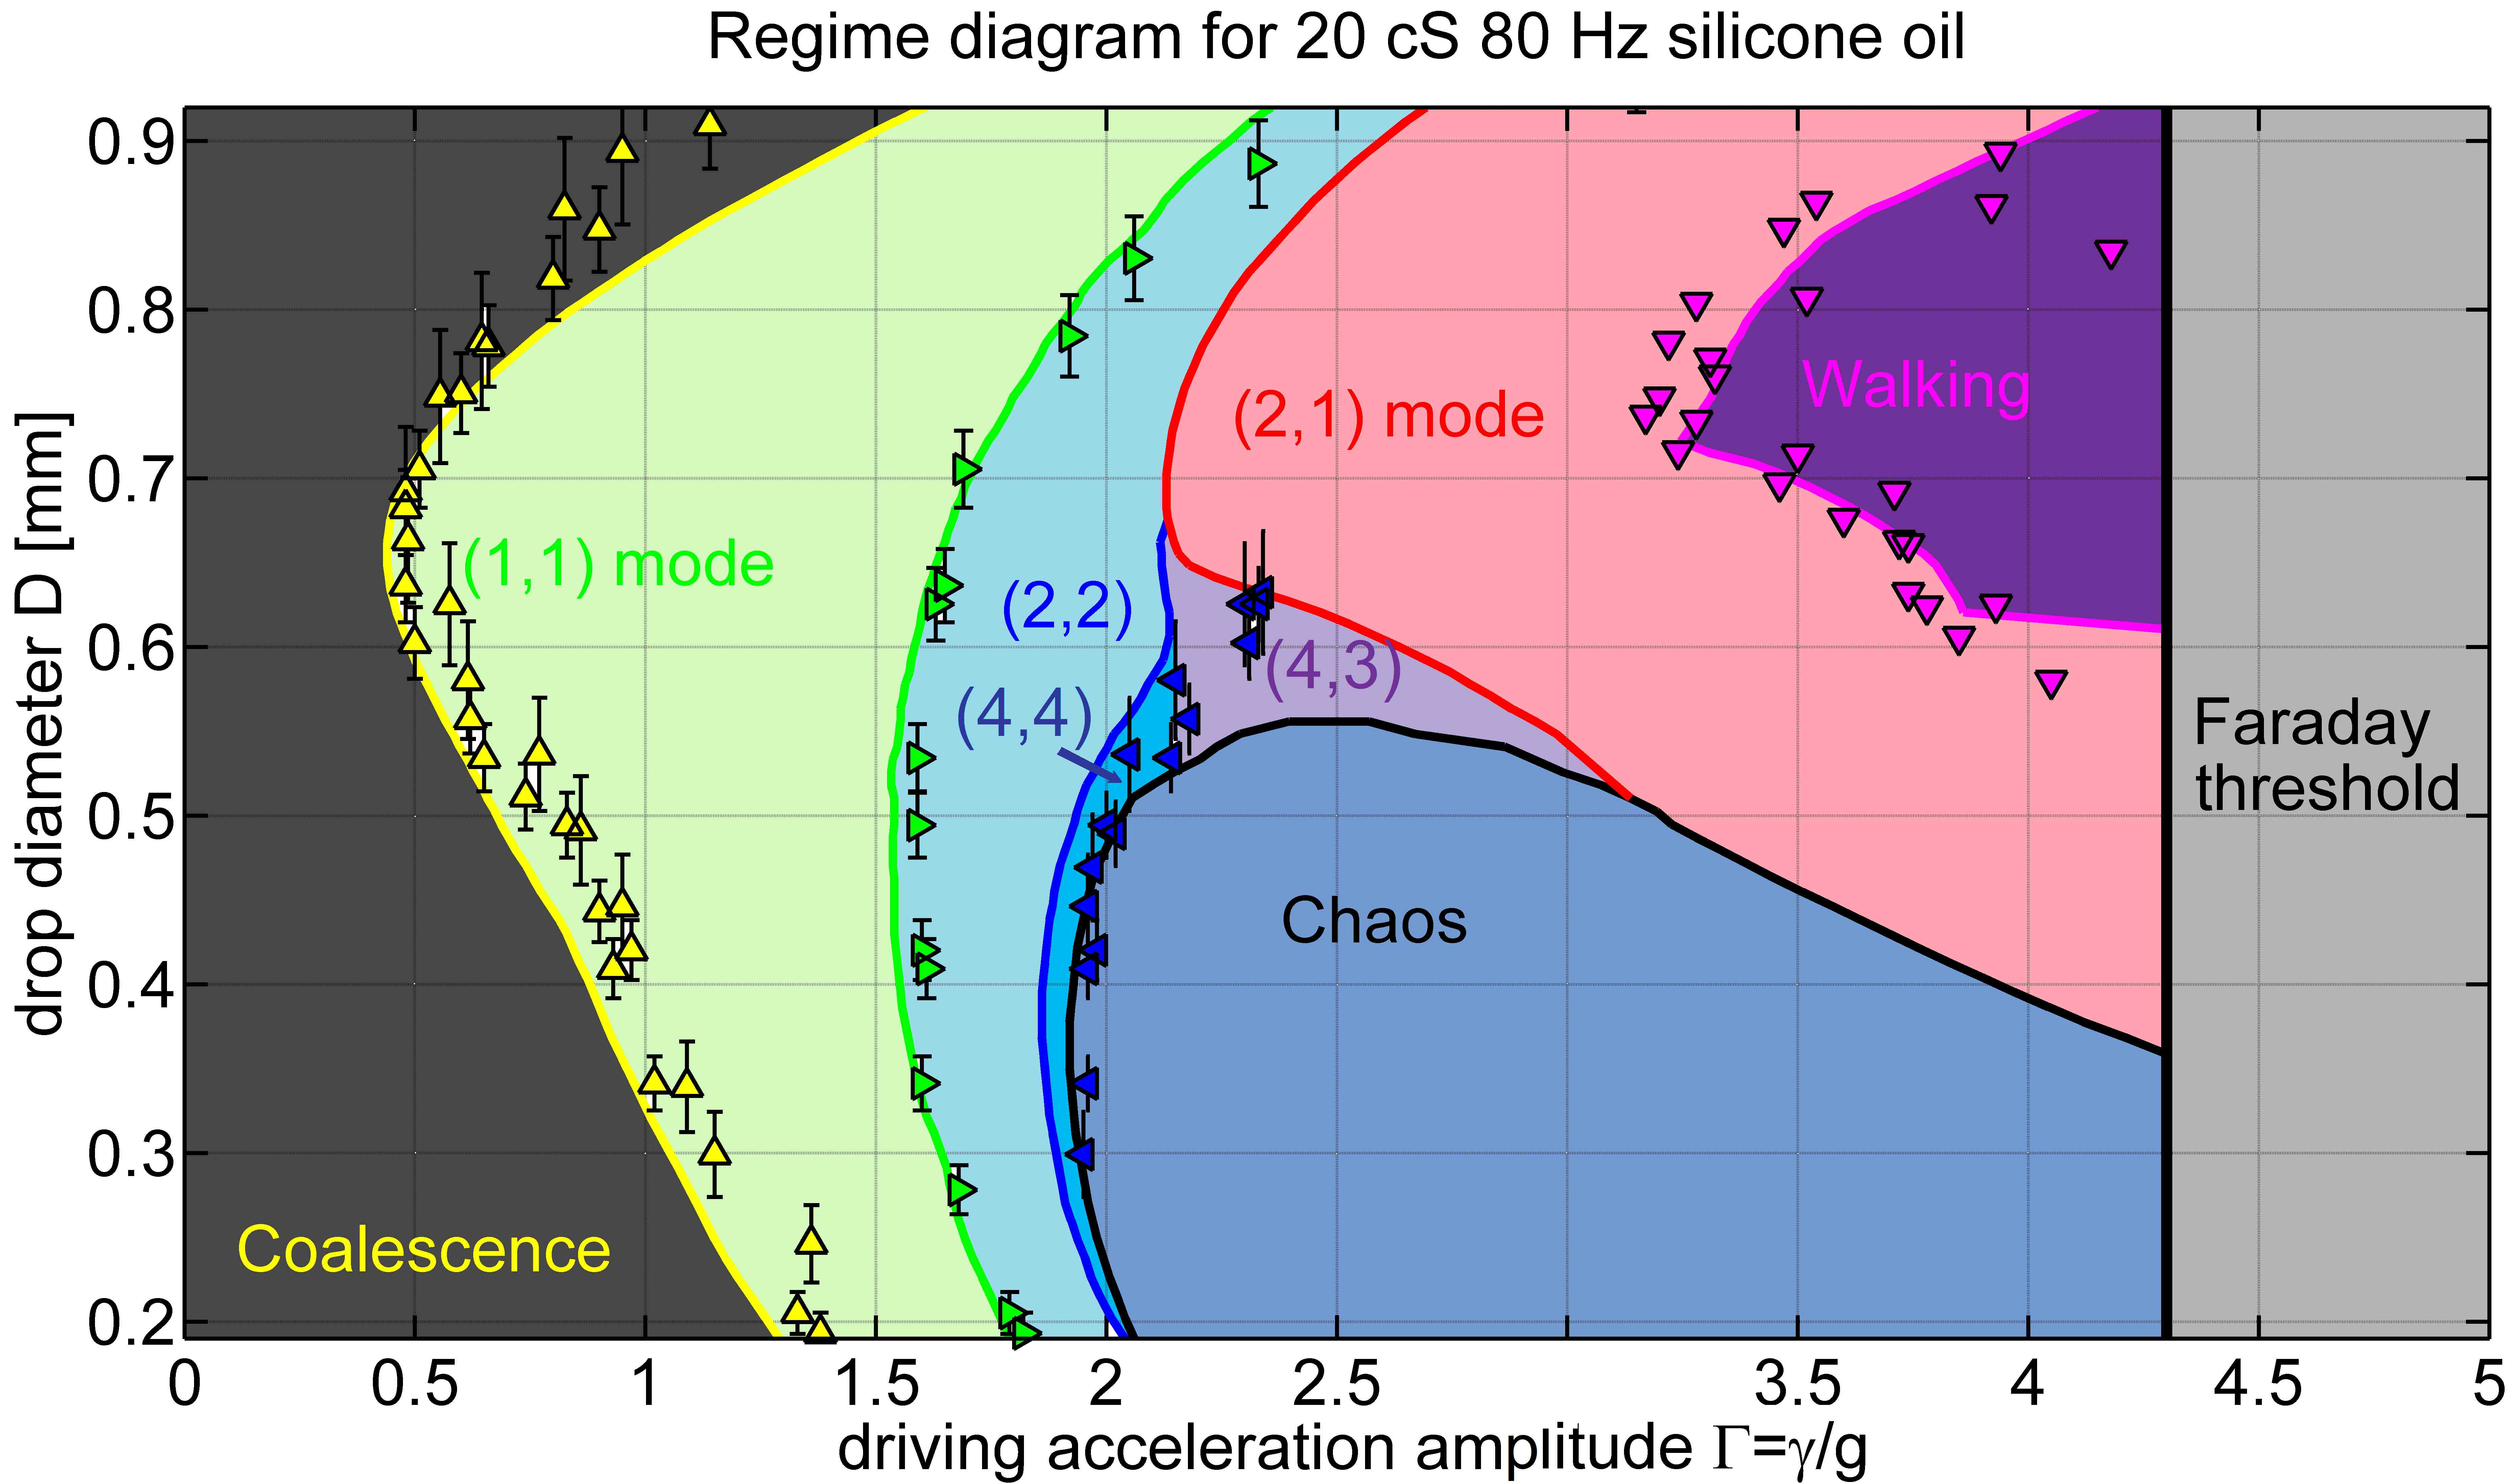
\includegraphics[scale=0.075]{Regime-Mega}
	     \caption{The different bouncing regimes for the oil drops of 20 cS silicon oil and at $f$ = $\omega / 2\pi$ = 80 Hz. The parameters ($m$,$n$) describe the droplet that bounces $n$ times in $m$ forcing periods. }
	 \label{regime}
	\end{figure}

The various modes seen in \refFig{regime} can be described by ($m$,$n$), where $n$ is the number to times the droplet contacts the surface over period $m/f$. For example, in the (1,1) mode, the droplet hits the oil bath once per driving period. In the (2,2) mode, the drop makes two bounces of differing heights. 
	       
            \subsection{Path Memory}
                        
            Path memory is a parameter that can be varied in this setup; it is essentially the damping of the system. Every time the droplet impacts the bath, it creates a radial traveling wave. Over the course of many bounces, a wavefield composed of a superposition of the many waves arises. In this way the wavefield ``remembers" previous interactions. Because droplet motion is influenced by the wavefield, controlling the damping of the wavefield will influence the path of the walker. The heavily damped system has a low memory, while undamped system correspends to higher memory. As one gets closer to the Faraday threshold, one achieves higher and higher memory because waves last for longer. The quantum like features of this experiment arise in the high-memory limit. (For more, Eddi et. al, 2011b: Information stored in Faraday waves.) 

            \subsection{Bound States}
            A bouncing droplet creates a damped wave that depends on the driving acceleration (${\gamma_m}/ g$) CITE: Protiere 2005. A periodic damped wave allows for two bouncers to form a ``bound state".  Starting far away from one another, the two droplets drift towards one another until a fixed distance $d_{0}^{bd}$. Increasing driving acceleration will decrease the value of $d_{0}^{bd}$. These bound bouncers form triangular lattices, and their periodicity is highly sensitive to the mass of the droplet. (LOOK AT EDDI ET ALL 2008).
            
            Walkers can also form bound states. Two walkers of the same size that are approaching one another can form an orbit around their center of mass. Between the two droplets is the fixed distance $d_{n}^{orb}$ given by
            
\begin{equation} \label{orbital}
d_{n}^{orb} = (n - \epsilon_0)\lambda_F
\end{equation}         
where $\epsilon_0$ is a fixed distance which is the same for all orbitals of these walkers (usually in the range $0.15 < \epsilon_0 < 0.25$ depending on droplet diameter), and $n = 1,2,3$... for drops that are in phase or $n = 1/2, 3/2, 5/2$... for drops out of phase. Orbiting periods are approximately porpotional to $d_{n}^{orb}$, which ends up meaning that the velocity of the orbiting walkers is a little less than the velocity of a free walker CITE: Protiere 2006. Orbiting of different sized droplets can also arise.      

            \subsection{Scattering States}
            Two identical walkers headed towards each other can form fixed orbits, or they can scatter. The droplets are deflected through their wavefields (they never actually make contact with one another)            
            \subsection{Single-Particle Diffraction}
In 2006 Couder and Fort showed that the system had properties that were strikinly similar to two famous and controversial quantum experiments (Couder and Fort, 2006). They were able to demonstrate that a single walker travelling through one slit seemed to have its direction altered seemingly randomly, before continuing forward on its new path. By statistically analyzing many trials, Couder and Fort showed that the histogram of the ``diffraction" actually resulted in a diffraction pattern strikingly similar to the single photon diffraction experiment performed by Taylor in 1909. 

Next, Couder and Fort added a second slit next to the first one. Now a single walker could pass through  one of two slits, and it was discovered that a histomgram of this data returned another diffraction pattern. This result is of course reminiscent of one of the most famous experiments in physics: Young's double slit diffraction with photons and electrons. 
    
Using a numerical simulation, Couder and Fort were able to reproduce similar results. 
    
As Couder and Fort mention in their paper: ``A discussion of the relation between these single-particle experiments and those concerning elementary particles is unavoidable." Important differences and similarities are then described between the quantum system and the quantum-like system. For the differences: we have a dissapative system, where energy is continually put in through the vibration of the tray; the particle can be followed;\footnote{C and F note that it'd be impossible to dectect the particle without disturbing it "by any means at its scale," like a bouy, for example. As the bouy floated it would interfere with the system by altering the wave pattern on the surface.} it's really effectively moving in two dimensions; the velocity is measurable; and the probability distributuion is linked with the wave amplitude (rather than it's intensity). And then of course, the similarities: an uncertainty priciple arises from the statistical data (and without knowledge of the actual paths followed by the walkers); and some others that were unclear...

Recently, Harris attempted to reproduce single slit interference. With better technology, new results were found. Using a looping guiding batt, trajectories were found to follow the same loop without deviating. Only at a very high memory were there chaotic paths.
	       \subsection{Tunneling}
	       The guiding wave field can be partially reflected off of an edge or even a change in depth of the oil bath. This effect can be seen when a walker is pushed back from a under-the-surface step, seemingly without any contact. In rare cases, the walker will actually tunnel across the step; that is, it will continue to walk along the surface of the oil bath and pass over the step without reflection. In the first experiment done by Eddi et al., they demonstrated tunneling by by building square ``corrals" of varying thicknesses. In the second experiment, they built a rhombus shape which forced the walker across the center of a rhombus. The barrier was placed perpendicular to the direction of travel of the walker, so that it would hit the wall directly rather than at an angle (as in the square corral). ``The tunneling probability decreases exponentially with the barrier width and increases as the Faraday threshold is approached." Eddi et. al also found that the probability of tunneling increased with the velocity of the walker. (For more, Eddi et. al 2009b: Unpredictable Tunneling of a classical wave-particle association.)
	       
	       
	        The unpredictability of the tunneling comes from the complex interatction between the drop and its guiding wave. 

\subsection{Motion in a Confined Geormetry}
By tracking the droplet as it bounces around the tray over a period of time, one can look at the overall statistical behavior of the droplet. Two experiments tracked walkers in an experimental coral (Harris and Bush, 2013, Harris et al. 2013) in the high-memory, chaotic motion regime. A histogram of the statistical data shows that the "probability of finding a walker at a given point in the corral is roughly prescribed by the amplitude of the Faraday wave mode of the cavity at the prescribed forcing frequency."

Quantum corral experiments performed by Crommie et al. (Crommie et al. 1993 a b) present similar findings. In the experiment, electrons were confined in a Cu(III) substrate using barriers of iron adatoms. Using tunneling spectroscopy, the electrons were found to have a specific resonances depending on the corral shape. As in the case of Harris' circular corral experiment where the corral and the Faraday wavelength, $\lambda_F$, dictate the wavelike statistical patter, in the quantum experiment the corral and the \textit{de Broglie} wavelength, $\lambda_{dB}$, dictate the form of the wavelike statistical pattern. 

\subsection{Walker Trajectories}
In the regime of walkers we have $R_e \sim 20$, $B_0 \sim 0.1$, and $W_e \sim 0.1$. For the millimeric walkers, the dominant force comes from impact of the curvature of the surface. Gilet and Bush (2009: Chaotic bouncing of a drop on a soap film, and the fluid trampline: droplets bouncing on a soap film) show that the surface of the vibrating oil can be modeled with a soap film, where the soap film acts like a linear spring. 

As the oil bath is forced up and down, a tiny droplet of oil will ``walk" across the surface. Mol\'{a}\v{c}ek and Bush have developed an equation of a droplet that describes the trajectory of the walking droplet, ignoring the verical dynamics by time averaging them out (cite: J. Mol\'{a}\v{c}ek and J. W. M. Bush, ``Drops walking on a vibrating bath: towards a hydrodynamic pilot-wave theory" J. FluidMech. 727, 612-647 (2013).). The trajectory of the walking droplet of mass $m$ at position $\textbf{x}(t) = (x(t),y(t))$ is given by
\begin{equation}
m \ddot{\textbf{x}} + D \dot{\textbf{x}} = -mg\nabla h(\textbf{x},t) 
\end{equation}
where $D$ describes the drag coefficient and $h(\textbf{x},t)$ describes the shape of the wavefield. Thus the second term describes the time averaged drag from both the flight and the impact of the droplet (as usual, depends on the velocity), and the third term describes the propulsive wave force resulting from drops landing on the inclined wave surface. 

The wavefield is quite complicated because it depends on the memory. For a single impact of a droplet, Oza et al. argue the surface wave can be approximated with an integral of a monochromatic radial Bessel function of the first kind

\begin{equation}
h(\textbf{x},t) = \frac{F}{T_F} \int_{-\infty}^{t} J_0 \frac{(k_F |\textbf{x}(t)-\textbf{x}(s)|)}{|\textbf{x}(t)-\textbf{x}(s)|} (\textbf{x}(t)-\textbf{x}(s))e^{-(t-s)/(T_F M_e)} ds
\end{equation}
with $F$ giving the wave force coefficient (estimated in the above source), $T_F$ describing the Faraday period, and $k_F$ describing the Faraday wave number determined by the Faraday wavelength $\lambda_F = 2π/k_F$ (integral from A. U. Oza, D. M. Harris, R. R. Rosales, and J. W. M. Bush, "Pilot-wave dynamics in a rotating frame: on the emergence of orbital quantization" J. Fluid Mech. 744, 404-429 (2014).). (Faraday was a popular guy.) Finally, that last term $M_e$ is the nondimensional memory parameter $M_e = T_d/[T_F(1-\gamma / \gamma_F)]$ (with $T_d$ being the unforced decay time).

\section{Experimental Setup}

\section{Bohmian Mechanics}

\subsection{Formalism}
\subsubsection{The Schroedinger Equation and $\psi$}

We begin with the Schoedinger equation

\begin{equation}
i \hbar \frac{\partial}{\partial t}\psi = \hat H \psi
\end{equation}
where $\hat H$ is the Hamiltonian and $\psi$ is the wavefunction. The Hamiltonian can be expanded (assuming there is no electric field) to give

\begin{equation}
\label{SE}
i\hbar\frac{\partial}{\partial t} \psi(\mathbf{x},t) = \left [ \frac{-\hbar^2}{2 m}\nabla^2 + V(\mathbf{x},t)\right ] \psi(\mathbf{x},t)
\end{equation}
where $V(\mathbf{x},t)$ is the potential energy of the system. The solution $\psi$ is of the form:

\begin{equation}
\psi(\mathbf{x},t) = R(\mathbf{x},t) e^{i S(\mathbf{x},t) / \hbar}
\end{equation}
where $S$ and $R$ are real. Plugging in our equation for $\psi$ into the Schoedinger equation (\refeq{SE}) will produce two separate equations: one giving the time derivative of $R$ and the second giving the time derivative of $S$. From these equations, a Hamilton-Jacobi equation can be written for a quantum system.
    Let's begin by computing the left hand side of \refeq{SE} in terms of $R$ and $S$.   

$$
\begin{align*}
i\hbar\frac{\partial}{\partial t} \psi(\mathbf{x},t) &= i \hbar\left(\frac{\partial R}{\partial t} e^{i S / \hbar} + R \frac{i}{\hbar}\frac{\partial S}{\partial t} e^{i S / \hbar}\right)
\\ &= i \hbar \left(\frac{1}{R} \frac{\partial R}{\partial t} + \frac{i}{\hbar}\frac{\partial S}{\partial t}\right) \psi(\mathbf{x},t) 
\\ &= \left(i \hbar \frac{1}{R} \frac{\partial R}{\partial t} - \frac{\partial S}{\partial t}\right) \psi(\mathbf{x},t)
\end{align*}
$$
Let's leave that alone for a little bit, while we focus on the right hand side of \refeq{SE}. Since it's a little more complicated, we will start with one term of the right hand side:

$$
\begin{align*}
\nabla^2 \psi(\mathbf{x},t)  &= e^{i S / \hbar} \nabla^2 R + \left(\frac{i}{\hbar}\right)^2 (\nabla S)^2 R e^{i S / \hbar} + \left(\frac{i}{\hbar}\right) R e^{i S / \hbar} (\nabla^2 S) + \left(\frac{2i}{\hbar}\right) (\nabla R \cdot \nabla S) R e^{i S / \hbar}
\\ &= \left(\frac{\nabla^2 R}{R} - \left(\frac{\nabla S}{\hbar}\right)^2  + \left(\frac{i \nabla^2 S}{\hbar}\right) + 2 i \left(\frac{\nabla R \cdot \nabla S}{\hbar}\right) \right) \psi(\mathbf{x},t) 
\end{align*}
$$

Now the hard part is done, and we can say that the right hand side of \refeq{SE} is given by 

$$
\begin{align*} 
\left [ \frac{-\hbar^2}{2 m}\nabla^2 + V(\mathbf{x},t)\right ]\psi(\mathbf{x},t) &= \left [-\frac{\hbar^2  \nabla^2 R}{2 m R} + \left(\frac{(\nabla S)^2}{2 m}\right)  - i \hbar \left(\frac{\nabla^2 S}{2 m}\right) - i \hbar \left(\frac{\nabla R \cdot \nabla S}{m}\right) + V(\mathbf{x},t) \right]\psi(\mathbf{x},t) 
\end{align*}
$$

Ok, now that we've got that done, the next part will be super easy. Starting with Schrodinger's equation and plugging in left and right hand sides we calulated seperately. 

$$
i\hbar\frac{\partial}{\partial t} \psi(\mathbf{x},t) = \left [ \frac{-\hbar^2}{2 m}\nabla^2 + V(\mathbf{x},t)\right ] \psi(\mathbf{x},t)
$$
$$
\left(i \hbar \frac{1}{R} \frac{\partial R}{\partial t} - \frac{\partial S}{\partial t}\right) \psi(\mathbf{x},t) =\left [-\frac{\hbar^2  \nabla^2 R}{2 m R} + \left(\frac{(\nabla S)^2}{2 m}\right)  - i \hbar \left(\frac{\nabla^2 S}{2 m}\right) - i \hbar \left(\frac{\nabla R \cdot \nabla S}{m}\right) + V(\mathbf{x},t) \right]\psi(\mathbf{x},t) 
$$
Now we can divide out $\psi$ from both sides
$$ 
i \hbar \frac{1}{R} \frac{\partial R}{\partial t} - \frac{\partial S}{\partial t} = -\frac{\hbar^2  \nabla^2 R}{2 m R} + \left(\frac{(\nabla S)^2}{2 m}\right)  - i \hbar \left(\frac{\nabla^2 S}{2 m}\right) - i \hbar \left(\frac{\nabla R \cdot \nabla S}{m}\right) + V(\mathbf{x},t)
$$
and group the imaginary numbers on the left side and the real numbers on the right side 
$$ i \hbar \frac{1}{R} \frac{\partial R}{\partial t} + i \hbar \left(\frac{\nabla^2 S}{2 m}\right) + i \hbar \left(\frac{\nabla R \cdot \nabla S}{m}\right) = \frac{\partial S}{\partial t} -\frac{\hbar^2  \nabla^2 R}{2 m R} + \left(\frac{(\nabla S)^2}{2 m}\right)  + V(\mathbf{x},t)
$$
Recall that both $S$ and $R$ are real. Note that the only way for all of the imaginary terms to equal all of the real terms is if they both equaled zero.
$$i \hbar \left(\frac{1}{R} \frac{\partial R}{\partial t} + \frac{\nabla^2 S}{2 m} + \frac{\nabla R \cdot \nabla S}{m}\right) = \left(\frac{\partial S}{\partial t} -\frac{\hbar^2}{2m}\frac{\nabla^2 R}{R} + \frac{(\nabla S)^2}{2 m}  + V(\mathbf{x},t) \right) = 0
$$
This then gives us two sepeate equations, one for the time derivative of $R$ and another for the time derivative of $S$.

\begin{equation}
\label{dR/dt}
\frac{\partial R}{\partial t} = -\frac{R}{2 m}\left(\frac{\nabla^2 S}{m}-2\nabla R \cdot \nabla S\right)
\end{equation}


\begin{equation}
\label{dS/dt}
\frac{\partial S}{\partial t} = \frac{\hbar^2}{2m}\frac{\nabla^2 R}{R} - \frac{(\nabla S)^2}{2 m} - V(\mathbf{x},t)
\end{equation}

What does this do for us? Both equations will provide helpful descriptions of our system.

\subsubsection{The Quantum Potential}

We can rewrite \refeq{dS/dt} in a provokative way 

\begin{equation}
\label{BohmHamiltonian}
- \frac{\partial S}{\partial t} = \frac{(\nabla S)^2}{2 m} + V(\mathbf{x},t) + \frac{\hbar^2}{2m}\frac{\nabla^2 R}{R}
\end{equation}
which should look suspiciously familiar. If I were to tell you that $\nabla S$ had units of momentum and $\partial S/\partial t$ units of energy, then this equation would look a lot like a Hamiltonian! The first term takes care of the kinetic energy, the second is the potential energy term, but we have this mysterious third term which we haven't ever encountered in classical mechanics. If we define this term as our ''quantum potential" 

\begin{equation}
\label{QuantumPotential}
U(\mathbf{x}) =  \frac{\hbar^2}{2m}\frac{\nabla^2 R}{R} = \frac{\hbar^2}{4m}\left[\frac{1}{2} \frac{\nabla^2 P}{P} - \frac{(\nabla P)^2}{P^2}\right] 
\end{equation}
then we really \textit{can} think of \refeq{BohmHamiltonian} as a Hamiltonian with an extra potential term thrown in to make it "quantum." Note that in cases where $\hbar$ is much smaller than the rest of the terms (i.e. not the quantum realm), then this quantum potential term goes away, and we are left with the regular Hamilton equation from classical mechanics. 

Recall that when writing a Hamiltonian, the potential terms govern the forces on the particle. For a conservative system, the force is given by F(x) = -$\partial U/\partial x$. If we include a quantum mechanical potential in our Hamiltonian, then this potential must cause a force on the paticle in addition to the one supplied by the $V(x)$ term. 


\subsubsection{Continuity Equation}
Plugging in the probability density $P(\mathbf{x},t) = R^2(\mathbf{x},t)$ into \refeq{dR/dt} also gives us something quite interesting.

MATH?

which we can finally express as 

\begin{equation}
\label{ProbCurrent}
\frac{\partial P}{\partial t} + \nabla \cdot \left( P \frac{\nabla S}{m} \right)
\end{equation}

In describing the quantum potential term it was mentioned that $\nabla S$ can be thought of as momentum, so then from our classical relationship between momentum and velocity  $\textbf{v}(\textbf{x},t)=\nabla S/m$ can be thought of as velocity. Then by defining the probability current as $j(\mathbf{x},t) = P\nabla S/m$ then we recover

\begin{equation}
\label{ProbCurrent}
\frac{\partial P}{\partial t} + \nabla \cdot j(\mathbf{x},t)
\end{equation}
known as the continuity equation! This tells us that $P$ is conserved over time.

\subsubsection{Finding $R$ and $S$}



    %\introduction command is provided as a convenience.
%if you want special chapter formatting, you'll probably want to avoid using it altogether
		
\chapter*{Introduction}
    \addcontentsline{toc}{chapter}{Introduction}
		\chaptermark{Introduction}
		\markboth{Introduction}{Introduction}
% The three lines above are to make sure that the headers are right, that the intro gets included in the table of contents, and that it doesn't get numbered 1 so that chapter one is 1.
\begin{quote}
	    ``While the founding fathers agonized over the question `particle' or `wave', de Broglie in 1925 proposed the obvious answer `particle' and `wave'... [t]his idea seems to me so natural and simple, to resolve the wave-particle dilemma in such a clear and ordinary way, that it is a great mystery to me that it was so generally ignored." -J. S. Bell
	    \end{quote}
	    
	    %"Six Possible Worlds of Quantum Mechanics" (1986), included in Speakable and Unspeakable in Quantum Mechanics (1987), p. 191

	    
	    %``For those who are not shocked when they first come across quantum theory cannot possibly have understood it." - Niels Bohr.


Quantum mechanics is perhaps one of the most counter-intuitive scientific theories in the history of the scientific method. At the atomic level, where quantum effects dominate, the laws that seem to govern our everyday world are no longer relevant. Determinism, the idea that every effect has a cause, is replaced with the idea that every action is probabilistic. A particle cannot be described by precise coordinates; instead, it is described using a wavefunction which provides a range of possible locations with associated probabilities. This probabilistic interpretation of quantum mechanics is known as the Copenhagen interpretation, and represents the most common form of rationalizing the radical, experimental observations of quantum mechanics. 

In 2005, Couder et al. showed that oil drops bouncing on a vertically vibrated fluid bath exhibit properties analogous to the paradoxical properties previously seen only at the quantum scale\rf{Couder2005b}.  The system operates at the macroscale, meaning that it is governed by the more ``intuitive" classical laws, but still behaves \textit{like} a quantum system. The accessibility of this experiment allows us to observe fundamental, ``quantum"-like phenomena in a way that is impossible at the nanoscale. For example, in quantum mechanics, one can never know the position \textit{and} the velocity of a particle, simply because it can never \textit{have} a perfectly defined position and velocity. In this experiment, however, the ``particle" can be easily seen at all times, so both its position and velocity can be easily tracked. 

    The behavior of the droplet system seems to agree with a theory of quantum mechanics proposed by Louis de Broglie in 1923 known as pilot-wave theory \rf{dB23,dB87}. Unlike the probabilistic viewpoint subscribed to by adherents of the Copenhagen interpretation, de Broglie's model asserts that the particle \textit{has} a precise location, and that the particle is pushed by a guiding or ``pilot" wave. The theory was extended by David Bohm in 1952 \rf{Bohm1952a,Bohm1952b}, but never caught on because it gained ``realism" (the idea that a particle is well defined at all times) at the expense of ``locality" (the idea of a universal speed limit where nothing, including information, can travel faster than the speed of light required by special relativity); a trade that is generally considered unfavorable by physicists.\footnote{The Copenhagen interpretation of quantum mechanics, by the way, is non-realist and non-local.} 
    
    De Broglie's original theory is underdeveloped, having remained relatively obscure for the better part of the last century. Since the predictions of the Copenhagen interpretation and de Broglie's theory are similar, experiments have done little to clarify the debate. As a result, the more developed Copenhagen school of thought holds its place as \textit{the} interpretation of quantum phenomena. 
    
     After taking a course in quantum mechanics, I found it difficult to truly believe some of the associated implications of the Copenhagen interpretation. I was seduced by some of the more obscure quantum methodologies that promised salvation from indeterminism and non-realism (such as Bohm or de Broglie's theories), and it was difficult from me to resist the opportunity to investigate analogs of these methodologies in an experimental setting. The bouncing droplet system, which serves as a hydrodynamic quantum analog and forms the backbone of this thesis, is introduced below. 
    
%Particle-wave association on a fluid interface (Protiere 2006).
	    \subsection*{Bouncing Droplets}
	    Though it had been observed for at least a century, the phenomena of droplets bouncing on a fluid bath was first explained by Jearl Walker in 1978\rf{Walker}. The investigations began with a simple droplet of water falling onto a bath of water and remaining just a second too long before coalescence.\footnote{It is often reported that this occurs in coffeemakers, as the coffee drips into the pot.} Walker discovered that by adding detergent to the water and vibrating the bath, he could extend the lifetime of the droplets from fractions of a second to several minutes. These droplets bounce at frequencies of around 50 Hz (50 bounces per second) and are very small, with a diameters of a millimeter or less. These two factors make it difficult to observe even the main mechanisms that drive the behavior. A key insight by Walker was that by flashing a strobe light at a frequency slightly slower than the rate of vibration of the bath, he could observe the droplet bouncing as if in slow motion.
	    
\begin{figure}[h!]
	\centering
	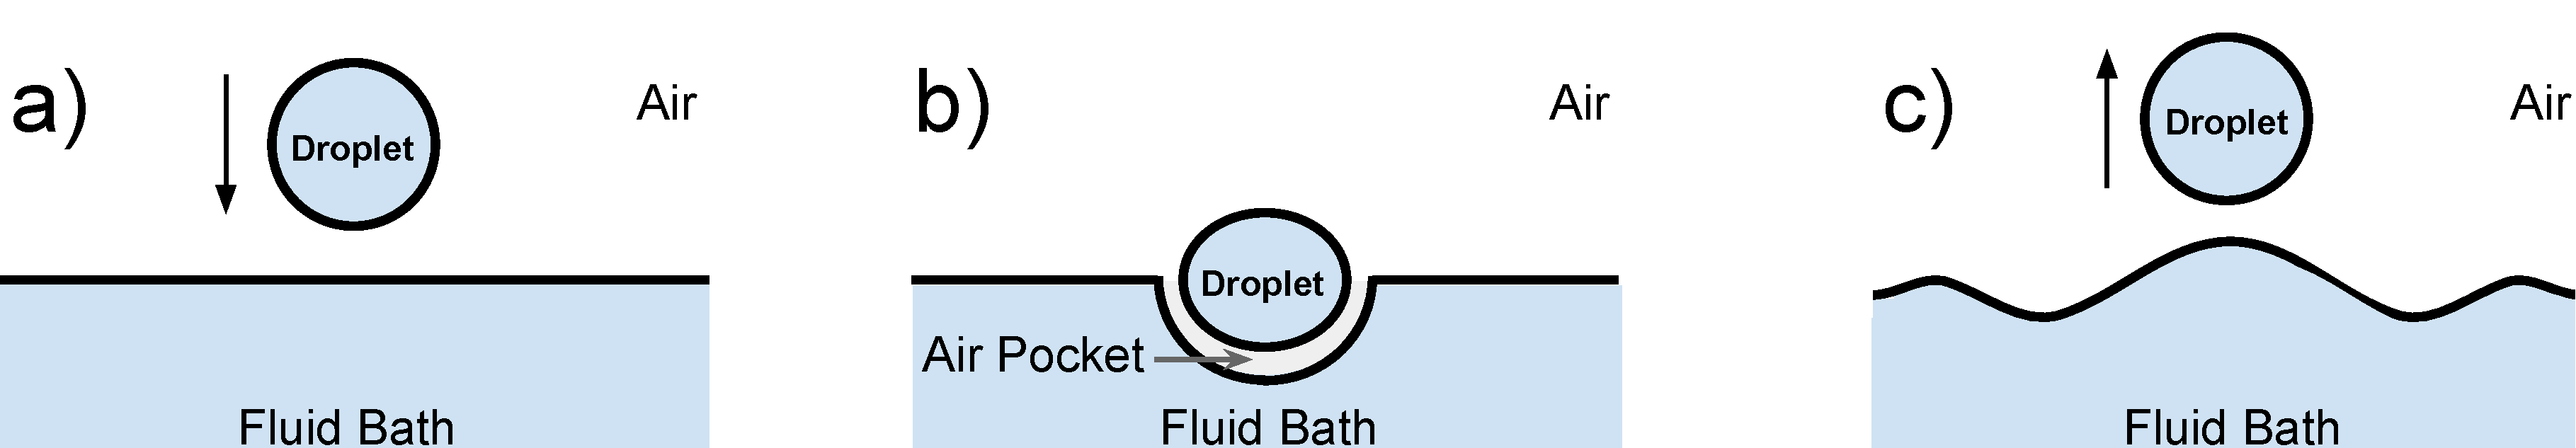
\includegraphics[scale=0.25]{BouncingDroplet.pdf}
	\caption{A depiction of a droplet bouncing on a bath of the same fluid. (a) A droplet falls onto a fluid bath. (b) A film of air gets trapped underneath the droplet. (c) The droplet bounces back up off of the cushion of air leaving behind waves that propagate radially.}
	\label{bounce}
\end{figure}
	    
	    Walker found that a trapped film of air kept the droplet and the bath from touching, as shown in \refFig{bounce}. That is, the droplet is bouncing on a layer of air that is being pushed out from under the droplet, but because the bounce happens so quickly, the fluid droplet and the fluid bath never touch. Walker concluded that the leakage rate of this trapped pocket of air depends on three factors: the surface tension of the fluid in the bath, the viscosity of the droplet and the fluid bath, and the viscosity of air. He found that the bath must be of uniform surface tension and free from floating particulate matter, since both could lead to coalescence. Higher viscosity fluids led to longer droplet lifetimes, since more viscous fluids make it more difficult for air to escape the gap between the drop and the bath. Finally, adjusting the frequency and the amplitudes of the vibrations also affected droplet lifetime.\footnote{Reedie Andrew Case ('92) wrote his thesis ``Oil on Troubled Water: The Extension of Floating Drop Lifetimes Due to Interface Vibration" where he looked at droplet lifetime as a function of vibrational frequency.}   
	     
	    More recent research showed that droplets of fluids like silicone oil can bounce indefinitely on a vibrating bath\rf{Couder2005a}. The long lifetime occurs not only because silicone oil has a high viscosity, but also because it has a \textit{low} surface tension. A low surface tension is beneficial because it makes the oil bath relatively immune to surfactants (e.g. detergent) or contamination that would otherwise make the surface tension nonuniform and lead the drop to coalescence. 

\subsection*{Faraday Waves}
	    The behavior of a fluid in a vertically vibrated bath can be controlled by adjusting the amplitude or the frequency of the vibration. Depending on a variety of factors (size of bath, fluid in bath, etc.) each system has a specific amplitude (given a specific frequency), which if surpassed, will produce standing surface waves called Faraday waves\rf{Faraday}.\footnote{Faraday waves were not actually discovered by Michael Faraday; in the footnotes of his paper he cites that they were first observed by Oersted, Wheatstone, Weber, and others. Faraday was just the first to study their behavior in detail.}~\footnote{Another Reed thesis, this one titled ``Good Vibrations: A Visual Exploration of Faraday Waves" by Alison Saunders empirically tested the mathematical Faraday wave model. } A vibrating bath below this critical amplitude, also known as the Faraday threshold, will have a quiescent surface. A bath driven at an amplitude greater than the Faraday threshold will have a turbulent surface with ripples and waves. An example of Faraday waves is shown in \refFig{faraday waves}. Adjusting the frequency above the Faraday threshold will change the size and shape of the Faraday waves. Note that Faraday waves can be created either by increasing the driving amplitude above a critical level, or adjusting frequency.	    
	    \begin{figure}[h!]
	\centering
	\includegraphics[scale=0.06]{Faraday.JPG}
	\caption{A picture of Faraday waves in a dish of water at $80~\mathrm{Hz}$.}
	\label{faraday waves}
\end{figure}

\subsection*{Walking Droplets}
	    
	A bouncing droplet will bounce differently depending on the frequency and amplitude of the vertical vibrations. If the parameters are set just below the Faraday instability, a curious motion arises: the droplet seems to ``walk" across the surface of the oil. The droplet is being pushed by its own ripples, a dual effort in which neither can exist without the other. In essence, the walker is both a particle and a wave; a conjunction reminiscent of the quantum scale. 
	  
\begin{figure}[h!]
	\centering
	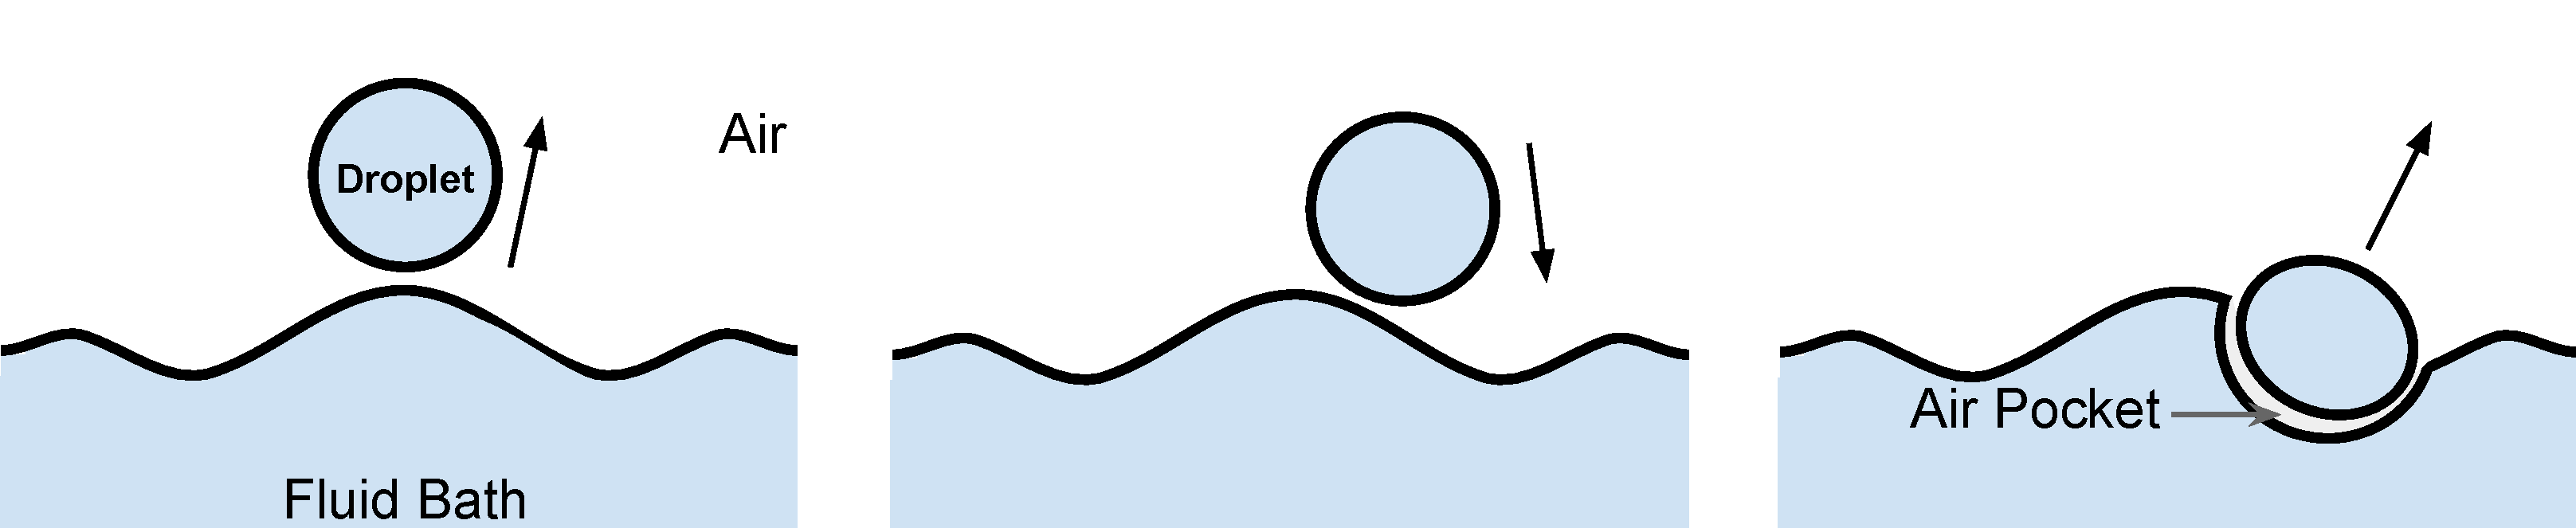
\includegraphics[scale=0.28]{Walking.pdf}
	\caption{A depiction of a droplet walking across a bath of the same fluid.}
	\label{bounce}
\end{figure}
	    
	  
\subsection*{Overview}	  
	  
	Recently, two main groups have been investigating the properties of this unique system. A group at Laboratoire Mati\`{e}re et Syst\`{e}mes Complexes (MSC) in Paris, France, headed by Yves Couder was the first to uncover some of the inherently ``quantum"-like behavior of bouncing droplets, in 2005~\cite{Couder2005b}. Since 2010, John Bush's group at MIT have created a mathematical model and performed their own investigations of the walker system. Couder, Bush, and others have shown that this system can reproduce double-slit single-particle interference \rf{double-slit}, tunneling \rf{tunneling}, quantized orbits \rf{Oza2014}, and many other ``quantum"-like effects \rf{pilot-wave}. 
		
	This thesis documents an experimental investigation into the ``tunneling" behavior of this bouncing droplet system. In this setting, tunneling occurs when the droplet interacts with a submerged barrier. Only one other study looks at this aspect~\cite{tunneling}, but falls short of completely examining the tunneling behavior, focusing on the effect of barrier width and not examining barrier height. I hope to add to the body of work in this subfield by studying how barrier height affects probability of tunneling.   
	
	This thesis is divided into three main chapters. \textbf{Chapter~1} describes the hydrodynamic quantum analog along with a brief survey of the relevant literature. \textbf{Chapter~2} describes the experimental design and explains the setup and the data acquisition procedures. \textbf{Chapter~3} presents the data from my experiments. Finally, the \textbf{Conclusion} highlights the results, summarizes the limitations, and suggests avenues for future study. 
    
    \chapter{Pilot-Wave Hydrodynamics}
\label{Ch1}

In this chapter I will present a brief survey of the literature describing  hydrodynamic quantum analogs, and discuss in more detail the tunneling experiments relevant to my investigation. Because the system was discovered in 2005, most of the literature examining this topic was written within the last decade.


\section{Oil Droplet System}
	    \label{parameters}
	       Consider a fluid of density $\rho$, viscosity $\nu$, and surface tension $\sigma$ in a bath of depth $H$. The bath is sinusoidally driven vertically with an amplitude $A_0$ at a frequency $f=\omega/{2\pi}$. By defining $\mathnormal{\gamma}=A_0\omega^2$, the effective gravity in the frame of reference of the bath is $g+\gamma~\mathrm{sin}(\omega t)$. The surface of fluid in the shaking tray remains quiescent for lower values of $\gamma$. However, if  $\gamma$ is increased above a certain threshold (by increasing $A_0$ or $f$), the surface becomes unstable leading to the appearance of standing surface waves called Faraday waves. We define this threshold as the \textbf{Faraday threshold}, $\gamma_\mathrm{F}$. The value of $\gamma_\mathrm{F}$ changes depending on the size and shape of the tray, the amount of fluid in the tray, as well as the properties of the fluid. 
	       
	   \begin{figure}[h]
	       \centering
	    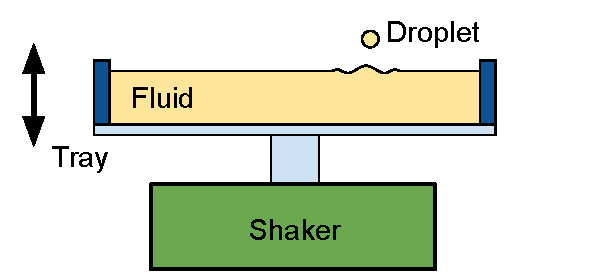
\includegraphics[scale=.80]{basicsetup.pdf}
	     \caption{A droplet bounces on a vertically vibrating fluid bath. The tray vibrates with an amplitude $A_0$ at frequency $f$.}
	 \label{basic}
	\end{figure}
	       
	    If we take a toothpick and break the surface of the vibrating oil bath, we form a droplet of oil of diameter $D$ as shown in \refFig{basic} that bounces on the surface for hours. The droplet bounces on a pocket of air, which is trapped beneath the droplet and the bath~\rf{Walker}. As the oil droplet bounces, it creates radially traveling waves that propagate outwards on an otherwise flat surface. The droplet will continue bouncing for a specific range of values of $\gamma$. For small $\gamma$, the forcing is not enough to sustain the droplet, and it quickly coalesces. Increasing $\gamma$ above the threshold for coalescence leads to a variety of different bouncing regimes until at $\gamma = \gamma_\mathrm{F}$ where Faraday waves emerge. Below $\gamma_\mathrm{F}$, the value of $\gamma$ also affects the range of the radial waves; for low $\gamma$, these waves quickly dissipate, but as $\gamma$ approaches $\gamma_\mathrm{F}$, they are sustained longer. We are interested in studying the region below the appearance of Faraday waves but above the region of coalescence. The range of the various parameters which allow for the existence of bouncing droplets are outlined in \refTab{approxlimits}. 
	      
	       \begin{table}[htdp] 
\caption[Basic Table 1]{Approximate limits for bouncing drop behavior. The value $g = 9.81~\mathrm{m/s}^{2}$ is the standard acceleration due to gravity. Adapted from \cite{pilot-wave}.} 
\begin{center} 
\begin{tabular}{c c c} 
\toprule 
  Parameter &  Lower Limit & Upper Limit \\
  \midrule
Viscocity $\nu$ (cSt) & 10 & 100 \\ 
Bath Depth $H$ (mm) & 4 & 10 \\
Frequency $f$ (Hz) & 20 & 150 \\
Amplitude $A_0$ (mm) & 0.1 & 1 \\
Drop Diameter $D$ (mm) & 0.6 & 1.0 \\
Forcing Acceleration $\gamma$ ($\mathrm{ms}^{-2}$) & 0.5$g$ & $\gamma_\mathrm{F} \approx 4.2g$ \\
\bottomrule 
\end{tabular}
\end{center}
\label{approxlimits} 
\end{table}	

\subsection{Faraday Waves}
Driving a fluid-filled tray with forcing acceleration $\gamma = \gamma_\mathrm{F}$ we see the appearance of standing surface waves known as Faraday waves. These waves oscillate with a  frequency $f_\mathrm{F} = f/2$ and an angular frequency $\omega_\mathrm{F} = 2\pi f_\mathrm{F}=\pi f$. For a fluid bath of density $\rho$, surface tension $\sigma$, and depth $H$, the standing wave and water dispersion relation:
\begin{equation} \label{dispersion}
\omega_\mathrm{F}^2 = \left(gk_\mathrm{F}+\frac{\sigma k_\mathrm{F}^3}{\rho}\right)\mathrm{tanh}(k_\mathrm{F}H),
\end{equation} 
can be used to find the wavelengths of standing waves at the Faraday threshold. This relates the angular Faraday frequency $\omega_\mathrm{F}$ to the Faraday wavenumber $k_\mathrm{F}$, where $g$ is the gravitational constant \rf{Kumar1996}. From the wavenumber, we can calculate the wavelength $\lambda_\mathrm{F}$ of the Faraday waves by the relation $\lambda_\mathrm{F}$ = $2\pi/k_\mathrm{F}$. Though we are interested in investigating the region $\gamma < \gamma_\mathrm{F}$ for which there are no standing surface waves, \refeq{dispersion} provides an estimate of the wavelength and frequency of the localized waves surrounding the droplet for the bouncing behavior. 


\subsection{Vibration Number}

In an experiment of this nature, one usually pours a specific volume of oil in the tray, fixing the values of $\nu$, $\sigma$, and $H$. One is then left with the option to adjust $\gamma$ which produces a range of droplet motions, including a slew of different stationary bouncing modes and linear or chaotic ``walking" trajectories (which are discussed in \refSect{sect:walking}). To categorize the various bouncing behaviors, we use the vibration number $V_i$, which takes into account many of the parameters of the experiment \rf{Molacek2013}. The vibration number is the ratio of the forcing frequency and the droplet's natural oscillation frequency $\omega_\mathrm{D}$ and is given by:
\begin{equation} \label{vibrationnumber1}
V_i = \frac{\omega}{\omega_\mathrm{D}.}
\end{equation}   
where $\omega_\mathrm{D}$ represents the oscillation frequency of a fluid droplet. Rather than remain a perfect sphere, the droplet stretches and contracts vertically as it bounces, and $\omega_\mathrm{D}$ describes the frequency of this motion. The oscillation frequency of a fluid droplet is defined as:
\begin{equation} \label{oscillationfrequency}
\omega_\mathrm{D} = 2\sqrt{\frac{2\sigma}{\rho D^3}},
\end{equation}   
where $\sigma$ is the surface tension, $\rho$ the density, and $D$ the diameter of the droplet \rf{lord}. Combining \refeqs{vibrationnumber1}{oscillationfrequency} we arrive at:
\begin{equation} \label{vibrationnumber2}
V_i = \frac{\omega}{2}\sqrt{\frac{\rho D^3}{2\sigma}},
\end{equation}   	       	       
a dimensionless parameter that captures the effects of the fluid's material properties, the tray's vibration, and the droplet's diameter. Depending on the vibration number $V_i$ and the driving strength $\gamma/g$, the droplets switch between different bouncing states as shown in \refFig{regime}. If we hold the working fluid and the driving frequency constant ($\sigma$, $\rho$, and $\omega$), then we can think of increasing $V_i$ as increasing droplet diameter $D$. 
	    
	    \begin{figure}[h]
	% the options are h = here, t = top, b = bottom, p = page of figures.
	% you can add an exclamation mark to make it try harder, and multiple
	% options if you have an order of preference, e.g.
	% \begin{figure}[h!tbp]
	       \centering
	    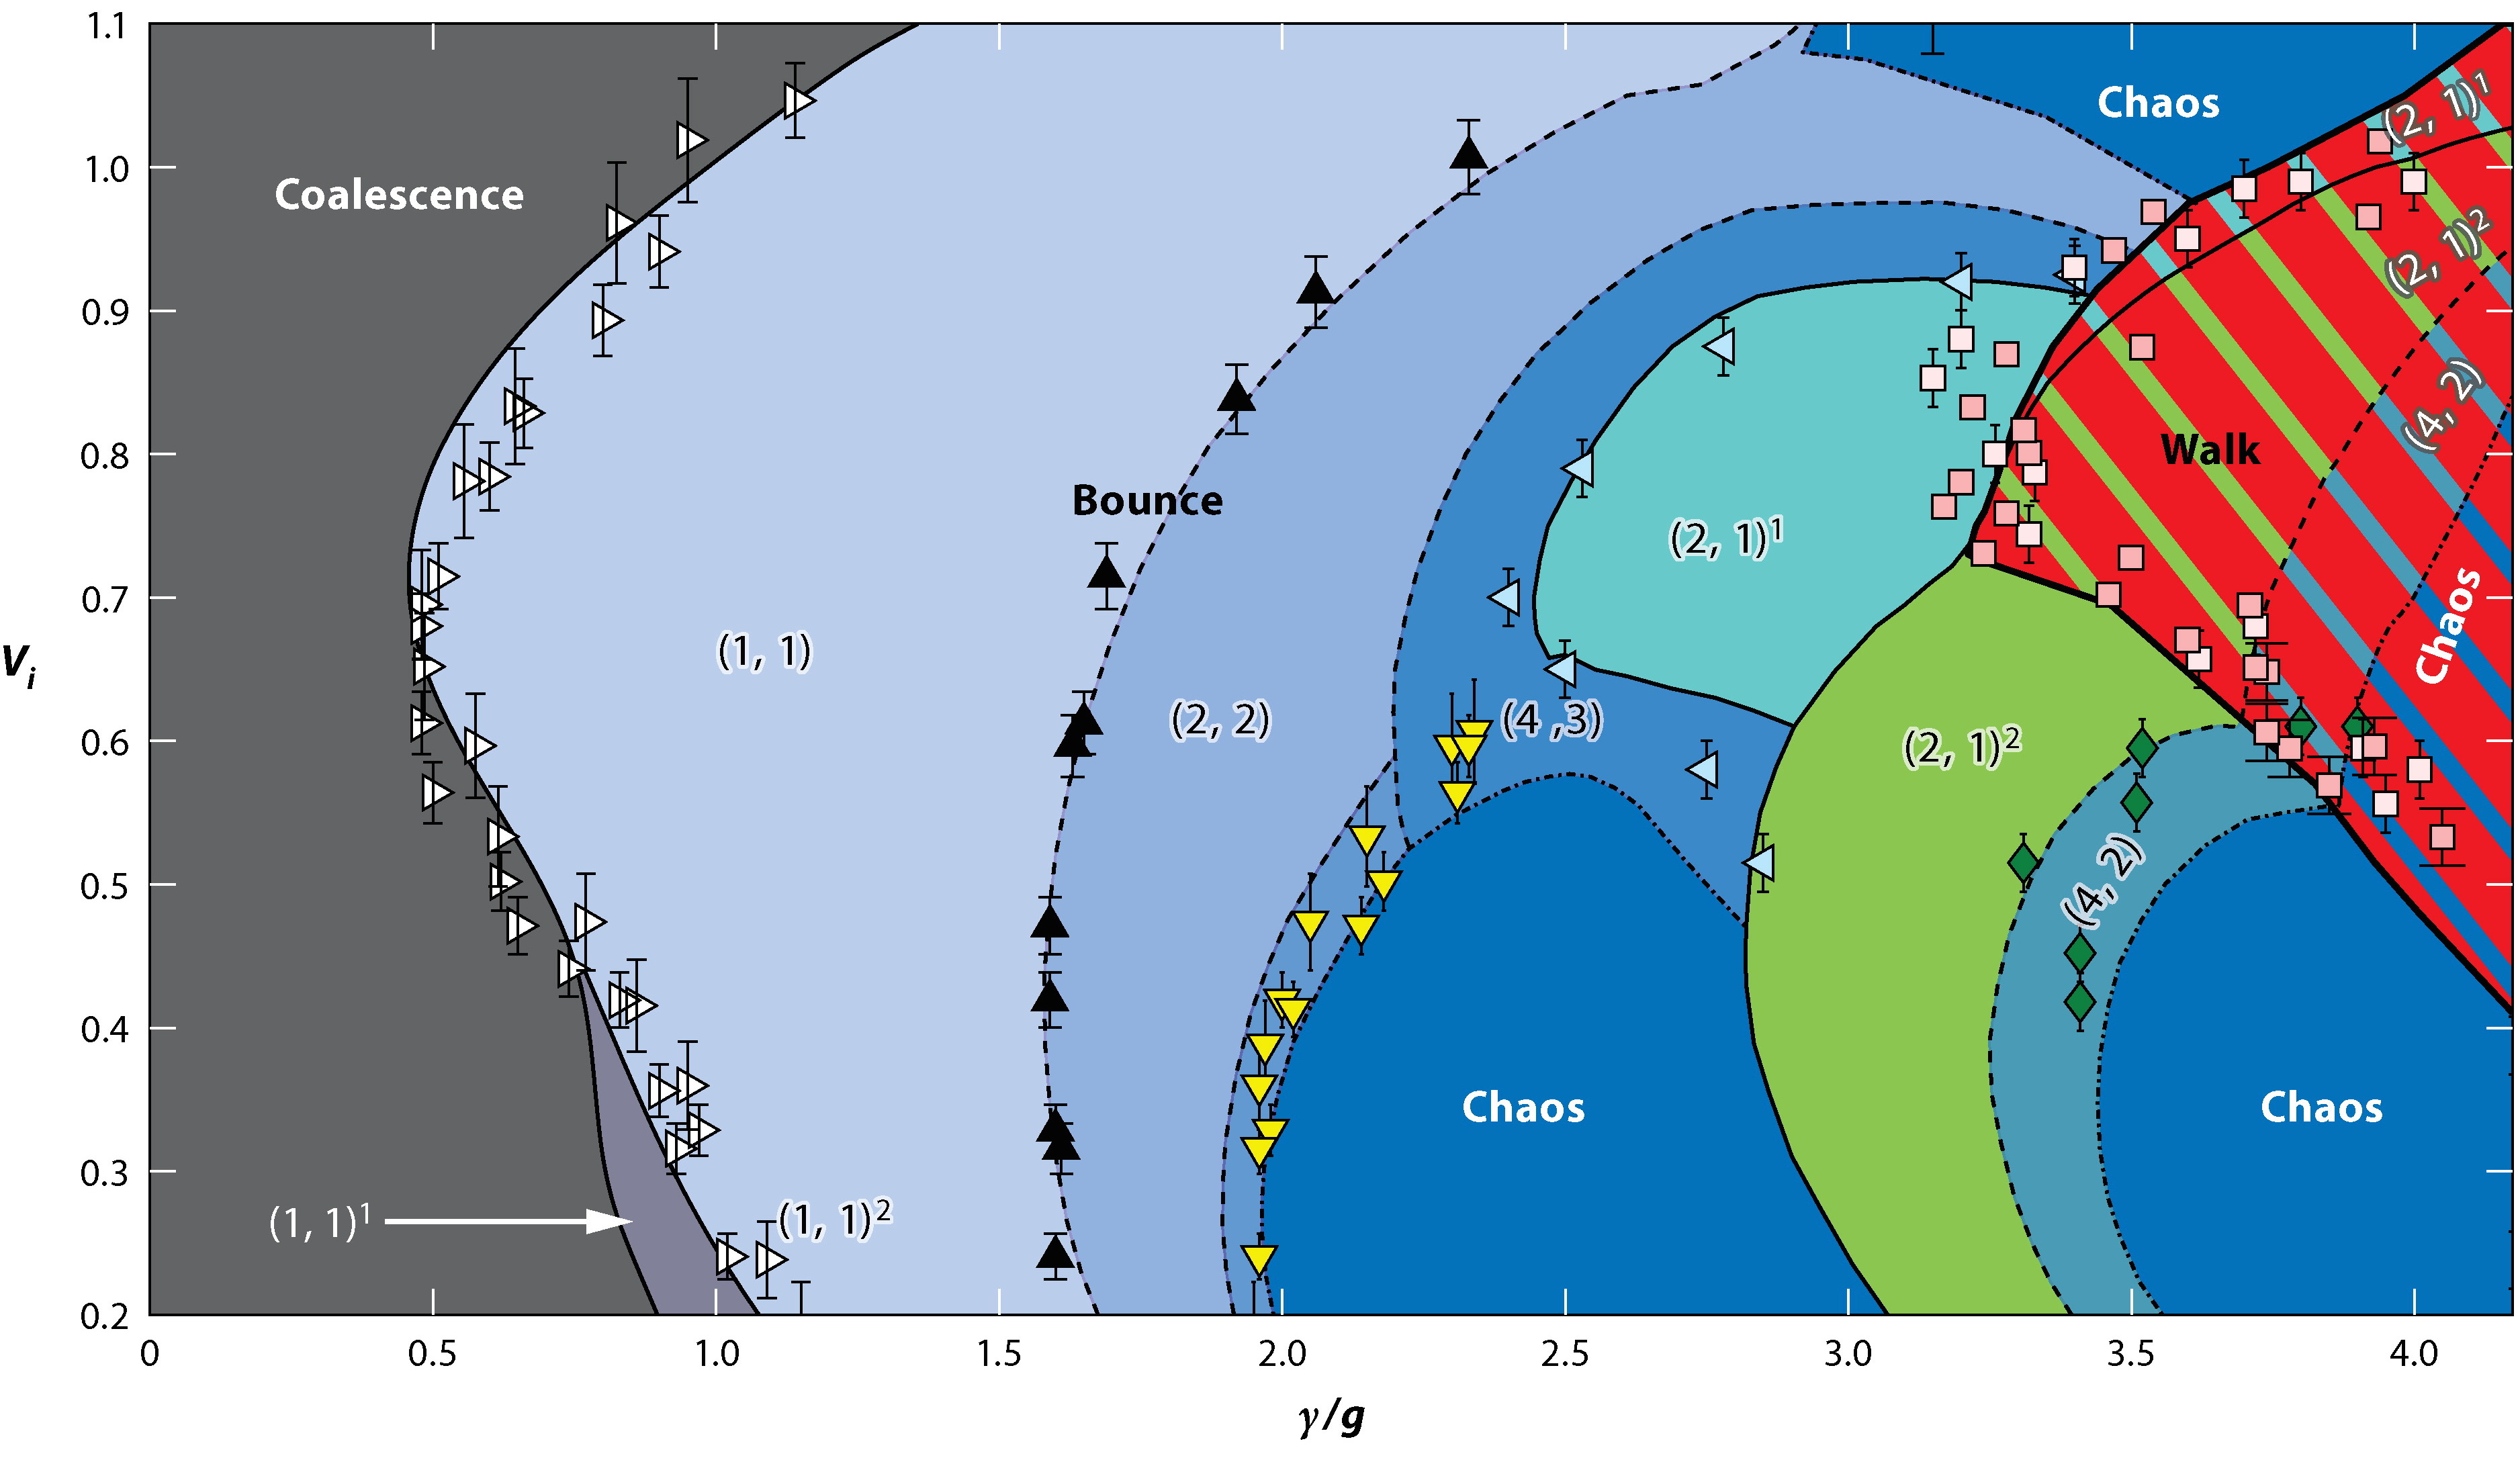
\includegraphics[scale=.1155]{vibrationnumber}
	     \caption{The different bouncing regimes for the oil drops of 20 cSt silicone oil at $f$ = $\omega / 2\pi$ = 80 Hz, characterized by the non-dimensional forcing amplitude $\gamma/g$ and the vibration number $V_i$. The solid colors represent the  modes predicted by a theoretical model~\rf{Molacek2013}, and the various points represent experimentally measured limits. The parameters $(m,n)^{i}$ describe a droplet that bounces $n$ times in $m$ forcing periods, where $i$ distinguishes modes with different mechanical energy. The Faraday threshold is $\gamma_\mathrm{F} = 4.2$. Adapted from J. W. M. Bush, Annu. Rev. Fluid Mech. \textbf{47}, 273 (2015).}
	 \label{regime}
	\end{figure}

The various modes seen in \refFig{regime} can be described by a pair of numbers~$m$ and $n$, where $n$ is the number of times the droplet contacts the surface over a time span $m/f$. For example, in the (1,1) ``bounce" mode, the droplet hits the oil bath once per up-and-down motion of the tray. In the (2,2) mode, the drop makes two bounces of differing heights for two driving periods. The ``chaos" regimes indicate that the bouncing of the droplet is chaotic and does not exhibit a periodic bouncing motion. The ``walk" regime describes a very particular kind of behavior in which the droplet moves forward as it bounces, seemingly walking across the surface. Like bouncing, walking also comes either the (2,1), (4,2), or chaotic modes. Finally, the ``coalescence" region demarcates the values for which the droplet coalesces with the bath.

The phase diagram shown in \refFig{regime} provides a valuable starting place for an experiment since it outlines the many possible states of the system, and where we can expect to find particular behaviors. We will now narrow our focus to only the walking regime, which is the focus of this thesis.

	        \subsection{Walking}
	        \label{sect:walking}
A walking droplet is a very specific type of bouncing droplet that arises between $\gamma_\mathrm{W}<\gamma<\gamma_\mathrm{F}$, where $\gamma_\mathrm{W}$ the the walking threshold. As the droplet bounces vertically on the vibrating fluid bath, the interaction with the wave it generated during its previous bounce gives it a slight horizontal motion. Thus, for every bounce, the droplet follows a parabolic trajectory. But because these droplets are bouncing at 40 times per second (or more) and the parabolic motion is periodic, the vertical oscillations are difficult to see. The apparent behavior that emerges is that of the droplet moving in a straight line along the surface of the fluid bath.             

 \begin{figure}[h]
	       \centering
	    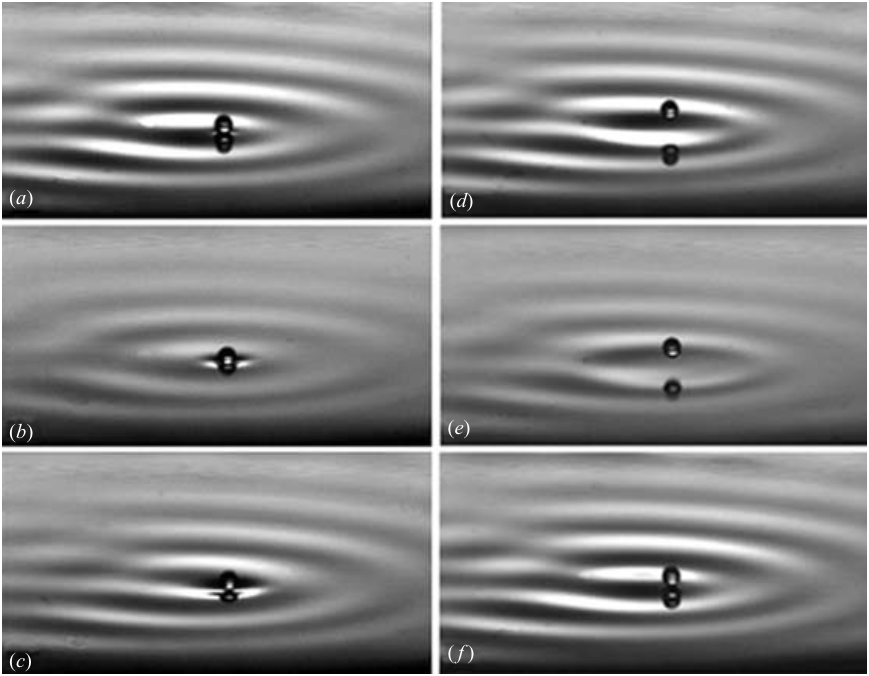
\includegraphics[scale=.495]{ProtiereWalkers}
	     \caption{%The series of pictures (a) - (c) show a droplet bouncing off of the slope of the localized wave, launching into the air, and then falling again on a new wave slope. This periodic process happens multiple times per second, giving the droplet the appearance of walking across the surface. Figure adapted from~\rf{Couder2005b}.
	    The series of pictures (a) - (f) show a walker over two forcing periods. The droplet bounces off of the slope of the localized wave, launching into the air, and then falls again on a new wave slope. This periodic process happens multiple times per second, giving the droplet the appearance of walking across the surface. Figure from S. Protiere et al., J. Fluid Mech. \textbf{554}, 93 (2006).
	     }
	 \label{Couderwalkers}
	\end{figure}
 
 
The horizontal component of the walking motion is due to the droplet landing slightly off center from the radial wave it produced in the previous bounce, as shown in \refFig{Couderwalkers}. At such close proximity to the Faraday threshold, the waves surrounding the droplet are not just regular ripples, but rather are like localized Faraday waves temporarily sustained by the vibrations before decaying away. The kinetic energy from the falling droplet is enough to perturb the unstable surface such that the waves appear, and then the energy introduced by the vertical forcing of the tray keeps these waves from damping out completely, as they would in an un-forced system. The value of $\gamma$ determines how long these local Faraday waves are sustained. As these waves interfere with one another they create an overall wave field that guides the droplet. This overall wave field is referred to as the \textbf{guiding wave} or the \textbf{pilot wave}. A \textbf{walker} is defined as a self-propelling droplet \textit{and} its guiding wave, since they are mutually interdependent; the droplet creates the guiding wave, and the guiding wave moves the droplet. The unique combination of the two components can result in novel interactions such as bound or scattering states.


%For example, as a walker approaches the wall of the tray, the droplet will slow down as it approaches and then--without touching the wall--walk off in the other direction. What's actually happening is that the guiding wave reflects off of the wall, which creates a new pilot-wave that pushes the droplet away from the wall. The defining quality illustrated in this example is that the droplet is apparently influenced by another feature without touching it, the interaction is happening with the guiding wave.

 \subsubsection{Bound States}

\begin{figure}[h]
	       \centering
	    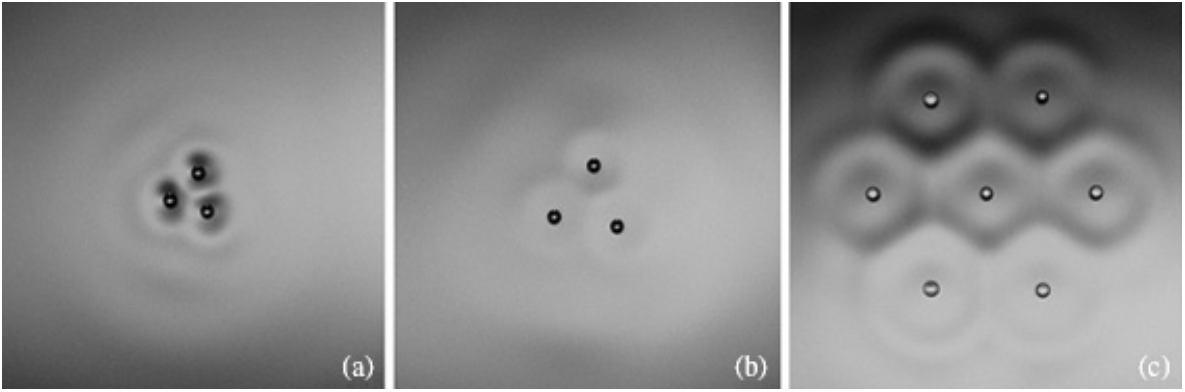
\includegraphics[scale=.366]{BoundedStates}
	     \caption{In (a), the trio of droplets organize themselves into a triangular lattice separated by distance $d_{0}^{bd}$. The forcing acceleration has been increased in (b), and the droplets are more spread out with a larger $d_{0}^{bd}$ value. Bound states can include a large number of bouncing droplets, as demonstrated by the 7 bouncing droplets shown in (c).   
	    Figure from S. Protiere et al., J. Phys.: Condens. Matter \textbf{17}, S3532 (2005). 
	     }
	 \label{bounded}
	\end{figure}
            A periodic damped wave allows for two bouncers to form a \textbf{bound state}: a configuration in which the droplets remain a fixed distance apart \rf{Protiere2005}.  Starting far away from one another, two droplets drift towards one another until a fixed distance $d_{0}^{bd}$. Increasing driving acceleration $\gamma$ decreases their separation distance $d_{0}^{bd}$ (\refFig{bounded}). These bound bouncers can form triangular lattices, although their periodicity is highly sensitive to the mass of the droplets. If the masses of the droplets differ, these configurations drift slowly and rotate because the waves produced by the larger droplet create an imbalanced wave field \rf{Eddi2008}. Finally, the droplets can bounce in phase with one another (they both land at the same time and reach their peaks at the same time) or completely out of phase with one another (as one lands, the other reaches its peak).
            
\begin{figure}[h]
	       \centering
	    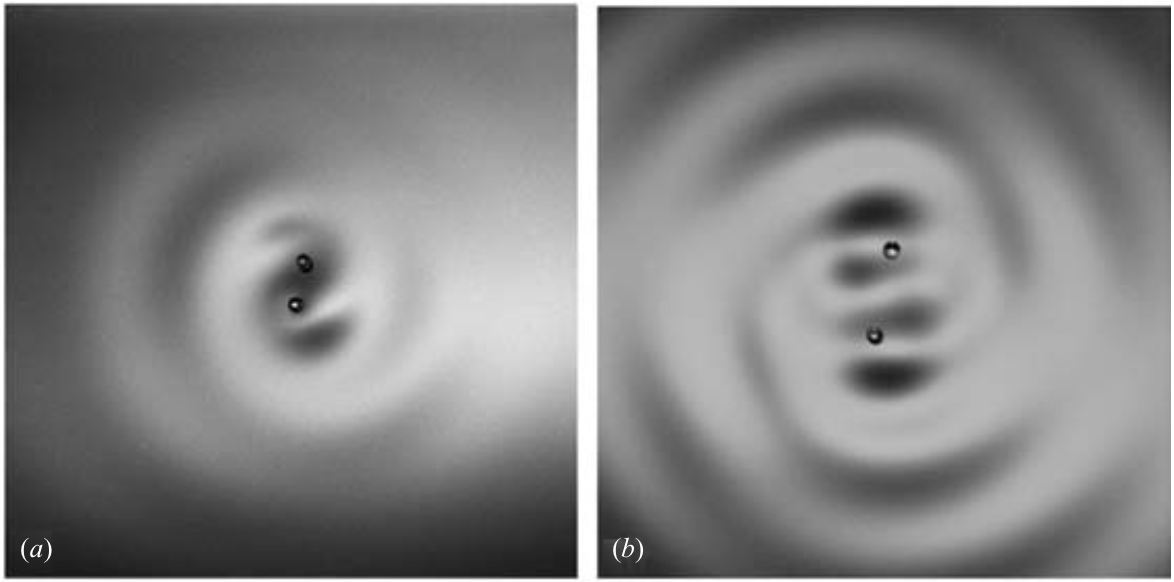
\includegraphics[scale=.33]{OrbitingProtiere2006}
	     \caption{ The figures show two droplets of equal size orbiting their center of mass. In (a) the droplets bounce out of phase with $n = 0.5$ and $d_{n}^{orb} =1.65~\mathrm{mm}$ whereas in (b) the droplets bounce in phase with  $n=1$ and  $d_{n}^{orb} = 3.7~\mathrm{mm}$.
	    Figure adapted from S. Protiere et al., J. Fluid Mech. \textbf{554}, 101 (2006). 
	     }
	 \label{orbiting}
	\end{figure}
 

            Walkers can also form bound states. Two walkers of the same size that are approaching one another can form an orbit around their center of mass as shown in \refFig{orbiting}. Between the two droplets is the fixed distance $d_{n}^{orb}$ given by          
\begin{equation} \label{orbital}
d_{n}^{orb} = (n - \epsilon_0)\lambda_F
\end{equation}         
where $\lambda_\mathrm{F}$ is the wavelength of the localized Faraday waves estimated by \refeq{dispersion}, $\epsilon_0$ is a fixed distance which is the same for all orbitals of these walkers (usually in the range $0.15 < \epsilon_0 < 0.25$ depending on droplet diameter), and $n = 1,2,3,...$ for drops that are in phase or $n = 1/2, 3/2, 5/2,...$ for drops out of phase. Orbiting periods are approximately proportional to $d_{n}^{orb}$, which ends up meaning that the velocity of the orbiting walkers is a little less than the velocity of a free walker \rf{Protiere2006}. 


            \subsubsection{Scattering States}
            Two identical walkers headed towards each other can form fixed orbits, or they can scatter. \textbf{Scattering} describes an interaction in which droplets are deflected through their wave fields, and never actually make contact with one another. Most of the interactions of a walker are scattering of some form. For example, if a single walker approaches the wall of the tray, it will never actually touch the wall. Instead, the guiding wave reflects off of the wall and modifies the wave field in such a way that the droplet will scatter in the opposite direction.           

%When two walkers interact with one another, their guiding waves interfere. Bouncing droplets will often organize themselves into stable configurations a specified distance apart. Increasing the forcing acceleration $\gamma$ will increase the separation between each droplet in the configuration. For walkers that 

%Walkers can travel anywhere from $5$ to $15~\mathrm{mm/s}$, depending on their size and on the driving acceleration $\gamma$ \rf{Protiere2005}.



 
            \subsection{Path Memory}
                        
            The system's proximity to the Faraday threshold is captured by a parameter called path memory. This captures the importance of damping in the system \rf{Eddi2011}. Every time the droplet impacts the bath, it creates a radial traveling wave. Over the course of many bounces, a guiding wave field composed of a superposition of the many waves arises. In this way the wave field ``remembers" previous interactions, but is at the same time being periodically ``updated" with every new bounce of the droplet. Because droplet motion is influenced by the wave field, controlling the damping of the wave field influences the path of the walker. 
            
For a bouncing droplet in which the guiding waves decay relatively quickly, the droplet can only be influenced by relatively recent waves. This kind of behavior is characterized as having a low memory. Conversely, a high memory system is one in which waves do not decay quickly; they propagate outwards and reflect off of the surfaces of the tray and interfere with the other waves produced by the droplet. As one gets closer to the Faraday threshold, one achieves higher and higher memory because waves last longer. The quantum-like features described here arise in the high-memory limit. 

The non-dimensional memory parameter is formally defined as:
$$M_e = \frac{T_\mathrm{d}}{T_\mathrm{F}(1-\gamma/\gamma_\mathrm{F})},$$
where $T_\mathrm{d}$ is the decay time of waves in the absence of vibration and $T_\mathrm{F}$ is the period of the Faraday waves ($T_\mathrm{F} = 1/f_\mathrm{F}$) \rf{Harris2013}. It will suffice to discuss memory as a fraction of the Faraday threshold $\gamma/\gamma_{F}$, since the fraction and $M_e$ are monotonically related. As the value of $\gamma/\gamma_{F}$ increases, we get closer to the Faraday threshold and $M_e$ increases. Eventually as $\gamma/\gamma_{F}$ approaches 1, the memory parameter approaches $+~\infty$. Thus, higher forcing $\gamma$ goes hand in hand with higher memory $M_e$. 

In practice, walking arises above a value of $\gamma/\gamma_{F}$ = 0.94, with more quantum-like phenomena arise at values of $\gamma/\gamma_{F} = 0.97$ and above \rf{Oza2014}. Deviations in memory $\gamma/\gamma_{F}$ as small as $\pm~0.01$ have been shown to have drastic differences in both long term and short term droplet behaviors \rf{Harris2013}.
            
            
\section{Bouncing Droplets as a Pilot-Wave Analog}   

The bouncing droplet system discussed above has remarkable similarities to a theoretical model of quantum mechanics. We start by introducing classical mechanics, which seeks to mathematically describe the motion of relatively large scale objects under action of forces. It was, until the late 19th century, physics. Physicists in the early 20th century, after a series of very puzzling experimental results, slowly began to realize that matter at the small scale behaved very differently than what they had been studying in the macroscale world. Quantum mechanics was developed, from the ground up, with the aim of mathematically describing this brave new world. As with any new behavior, a variety of theoretical explanations with mathematically different foundations were tossed around, until, at the 1927 Solvay conference, the Copenhagen interpretation of quantum mechanics emerged. The Copenhagen interpretation was spearheaded by Niels Bohr and Werner Heisenberg, and provides a way of interpreting the mathematics of quantum mechanics. This interpretation is fundamentally probabalistic. In the modern day, most physicists teach and preach the Copenhagen interpretation of quantum mechanics because it is in excellent agreement with experiment and it also is more developed than other interpretations.

The oil droplet system is classical, but it is unique in that it is a classical system that behaves \textit{like} a quantum system. Experimentally, it exhibits a variety of counter-intuitive interactions similar to those seen in quantum mechanical systems \rf{Brady}. These include single particle double slit diffraction \rf{double-slit}, quantized orbits, tunneling (discussed in \refSect{sect:tunneling}) \rf{tunneling}, and others \rf{pilot-wave}. These unique features stem from the \textbf{particle-wave duality}, a central concept in quantum mechanics: the idea that a particle can behave like a particle in some circumstances and like a wave in others. In the hydrodynamic pilot-wave system, this is represented by the walker which is both a droplet and a wave.

The oil droplet system is slightly different than the actual quantum conception  since the walker is a droplet \textit{and} a wave, while the Copenhagen interpretation describes an electron (for example) as a particle \textit{or} a wave. In this sense the oil droplet system is not analogous to the Copenhagen interpretation of quantum mechanics. However, it bears remarkable resemblance to a theory proposed by L. de Broglie in 1923, the so-called ``double solution" theory \rf{dB23}. De Broglie proposed that the particle is guided by two waves: a pilot wave created by internal particle oscillations that affects the immediate behavior of the droplet (i.e. the localized Faraday waves) and evolves according to the Klein-Gordon equation, and a wave outlined by the Schr\"{o}dinger equation that describes the long term statistical behavior of the droplet's location over time (discussed in \refSect{sec:longterm}) \rf{dB87}. The second statistical wave describing the long term motion of the particle in de Broglie's theory is the very same wave that describes the particle's probable location using the Copenhagen interpretation, but because of de Broglie's extra pilot wave, the same wave is interpreted differently. Unfortunately, because de Broglie could never find the equation of the pilot wave, he could not proceed with his theory and it fell into obscurity. His theory was picked up and modified by David Bohm in 1952 \rf{Bohm1952a,Bohm1952b}, who combined the statistical wave and the guiding wave into a single wave. By combining the two waves, Bohm's formulation loses its relevance to the bouncing droplet system.

It is worth noting that there are a few differences between the hydrodynamic system and an actual quantum system. First of all is the scale; the bouncing droplet system moves under the laws of the macroscopic world. Secondly, the hydrodynamic system is dissipative (waves are damped) and sustained only through continuous energy input (constantly being vibrated), so it is not a conservative system. With that said, it is still worth comparing the two since they appear similar in many other respects.

Despite these differences, it is worth investigating the hydrodynamic pilot-wave analogs in greater detail. We will narrow our focus once again, and investigate the tunneling behavior of this system, which describes the droplet's interaction with subsurface barriers. The following section explains tunneling in quantum mechanics, and the analogous behavior in the droplet system. 

%and eventually picked up by David Bohm who in 1952 modified them to create Bohmian mechanics. This modification, which made it quite popular in the undeground physics community, lost some of the original aspects of de Broglie's theory. As such, it is much closer 

%A fundamental concept in quantum mechanics is the idea of \textbf{wave-particle duality}, that an particle can often times behave like a wave and other times behave like a point mass. The particle dissonance is highlighted in the double slit experiment which was finally conducted in 1974, though it's outcome already been predicted with other, less precise experiments \rf{Italins}. When light is sent through a two slits, the resulting pattern is one of interference. When an electron is aimed at the two slits, it can go through one of the two slits or it can bounce back. The dissonance arises when the experimenter takes a measurement of which slit the particle went through. If the measurement is made and the experimenter knows which slit the electron passed through, then the resulting pattern is like that of a point mass traveling through. If the measurement is not made, then the behavior of a single electron is like that of interfering waves. How can it be, that when we make a measurement of something, we change the way an electron interacts with the world?



%There is the also story we tell ourselves, conceptually and to some extent mathematically, what exactly is going on during these processes. These interpretations of quantum mechanics is what causes all the fuss. As Niels Bohr famously said: ``For those who are not shocked when they first come across quantum theory cannot possibly have understood it" \rf{?}. This is because the 

 %            \subsection{Single-Particle Diffraction}
%In 2006 Couder and Fort showed that the system had properties that were strikingly similar to two famous and controversial quantum experiments \cite{double-slit}. They were able to demonstrate that a single walker traveling through one slit seemed to have its direction altered seemingly randomly, before continuing forward on its new path. By statistically analyzing many trials, Couder and Fort showed that the histogram of the ``diffraction" actually resulted in a diffraction pattern strikingly similar to the single photon diffraction experiment performed by Taylor in 1909. 

%Next, Couder and Fort added a second slit next to the first one. Now a single walker could pass through  one of two slits, and it was discovered that a histogram of this data returned another diffraction pattern. This result is of course reminiscent of one of the most famous experiments in physics: Young's double slit diffraction with photons and electrons. 
    
%Using a numerical simulation, Couder and Fort were able to reproduce similar results. 
    
%As Couder and Fort mention in their paper: ``A discussion of the relation between these single-particle experiments and those concerning elementary particles is unavoidable." Important differences and similarities are then described between the quantum system and the quantum-like system. For the differences: we have a dissipative system, where energy is continually put in through the vibration of the tray; the particle can be followed;\footnote{C and F note that it'd be impossible to detect the particle without disturbing it "by any means at its scale," like a bouy, for example. As the bouy floated it would interfere with the system by altering the wave pattern on the surface.} it's really effectively moving in two dimensions; the velocity is measurable; and the probability distribution is linked with the wave amplitude (rather than it's intensity). And then of course, the similarity: an uncertainty principle arises from the statistical data (and without knowledge of the actual paths followed by the walkers). %and some others that were unclear...

%Recently, Harris attempted to reproduce single slit interference. With better technology, new results were found. Using a looping guiding batt, trajectories were found to follow the same loop without deviating. Only at a very high memory were there chaotic paths.

\subsection{Long Term Droplet Behavior}
\label{sec:longterm}


%\subsubsection{Confined Electrons}
%By arranging 48 iron atoms in a ring on top of a copper(III) substrate, Crommie et al. made a quantum ``corral" that confined electrons to a circle of radius $73~\mathrm{\r{A}}$ \rf{Crommiea}\rf{Crommieb}. 

%Quantum corral experiments performed by Crommie et al. (Crommie et al. 1993 a b) present similar findings. In the experiment, electrons were confined in a Cu(III) substrate using barriers of iron adatoms. Using tunneling spectroscopy, the electrons were found to have a specific resonances depending on the corral shape. As in the case of Harris' circular corral experiment where the corral and the Faraday wavelength, $\lambda_F$, dictate the wavelike statistical patter, in the quantum experiment the corral and the de Broglie wavelength, $\lambda_{dB}$, dictate the form of the wavelike statistical pattern. 



%\subsubsection{Confined Droplets}



Constraining a walker to a circular region, Harris et al. tracked the motion of the walker over a long period of time \cite{Harris2013}. In the high-memory, chaotic motion regime, the droplet was allowed to walk freely while its position was tracked (\refFig{stat}(a)) and translated into the histogram (\refFig{stat}(b)). The histogram provides the probability of finding the walker at a specific location within the corral, and recovers the shape of the Faraday wave that occurs at the Faraday threshold. This histogram serves the same purpose as de Broglie's statistical wave described by the Schr\"{o}dinger equation. In the Copenhagen interpretation of quantum mechanics, however, this statistical wave (called the wavefunction) fully defines the particle. 

%The histogram generated by Harris et al. looks very similar to the Faraday standing wave that occurs at $\gamma_\mathrm{F}$, and has the characteristic wavelength $\lambda_\mathrm{F}$. At the quantum scale, as shown by an experiment conducted by Crommie et al., a similar wave emerges for an electron confined to a circular geometry. Rather than being a wave described by $\lambda_\mathrm{F}$, it was found that the wave had a wavelength of $\lambda_\mathrm{db}$, or a de Broglie wavelength.
\begin{figure}[h]
	       \centering
	    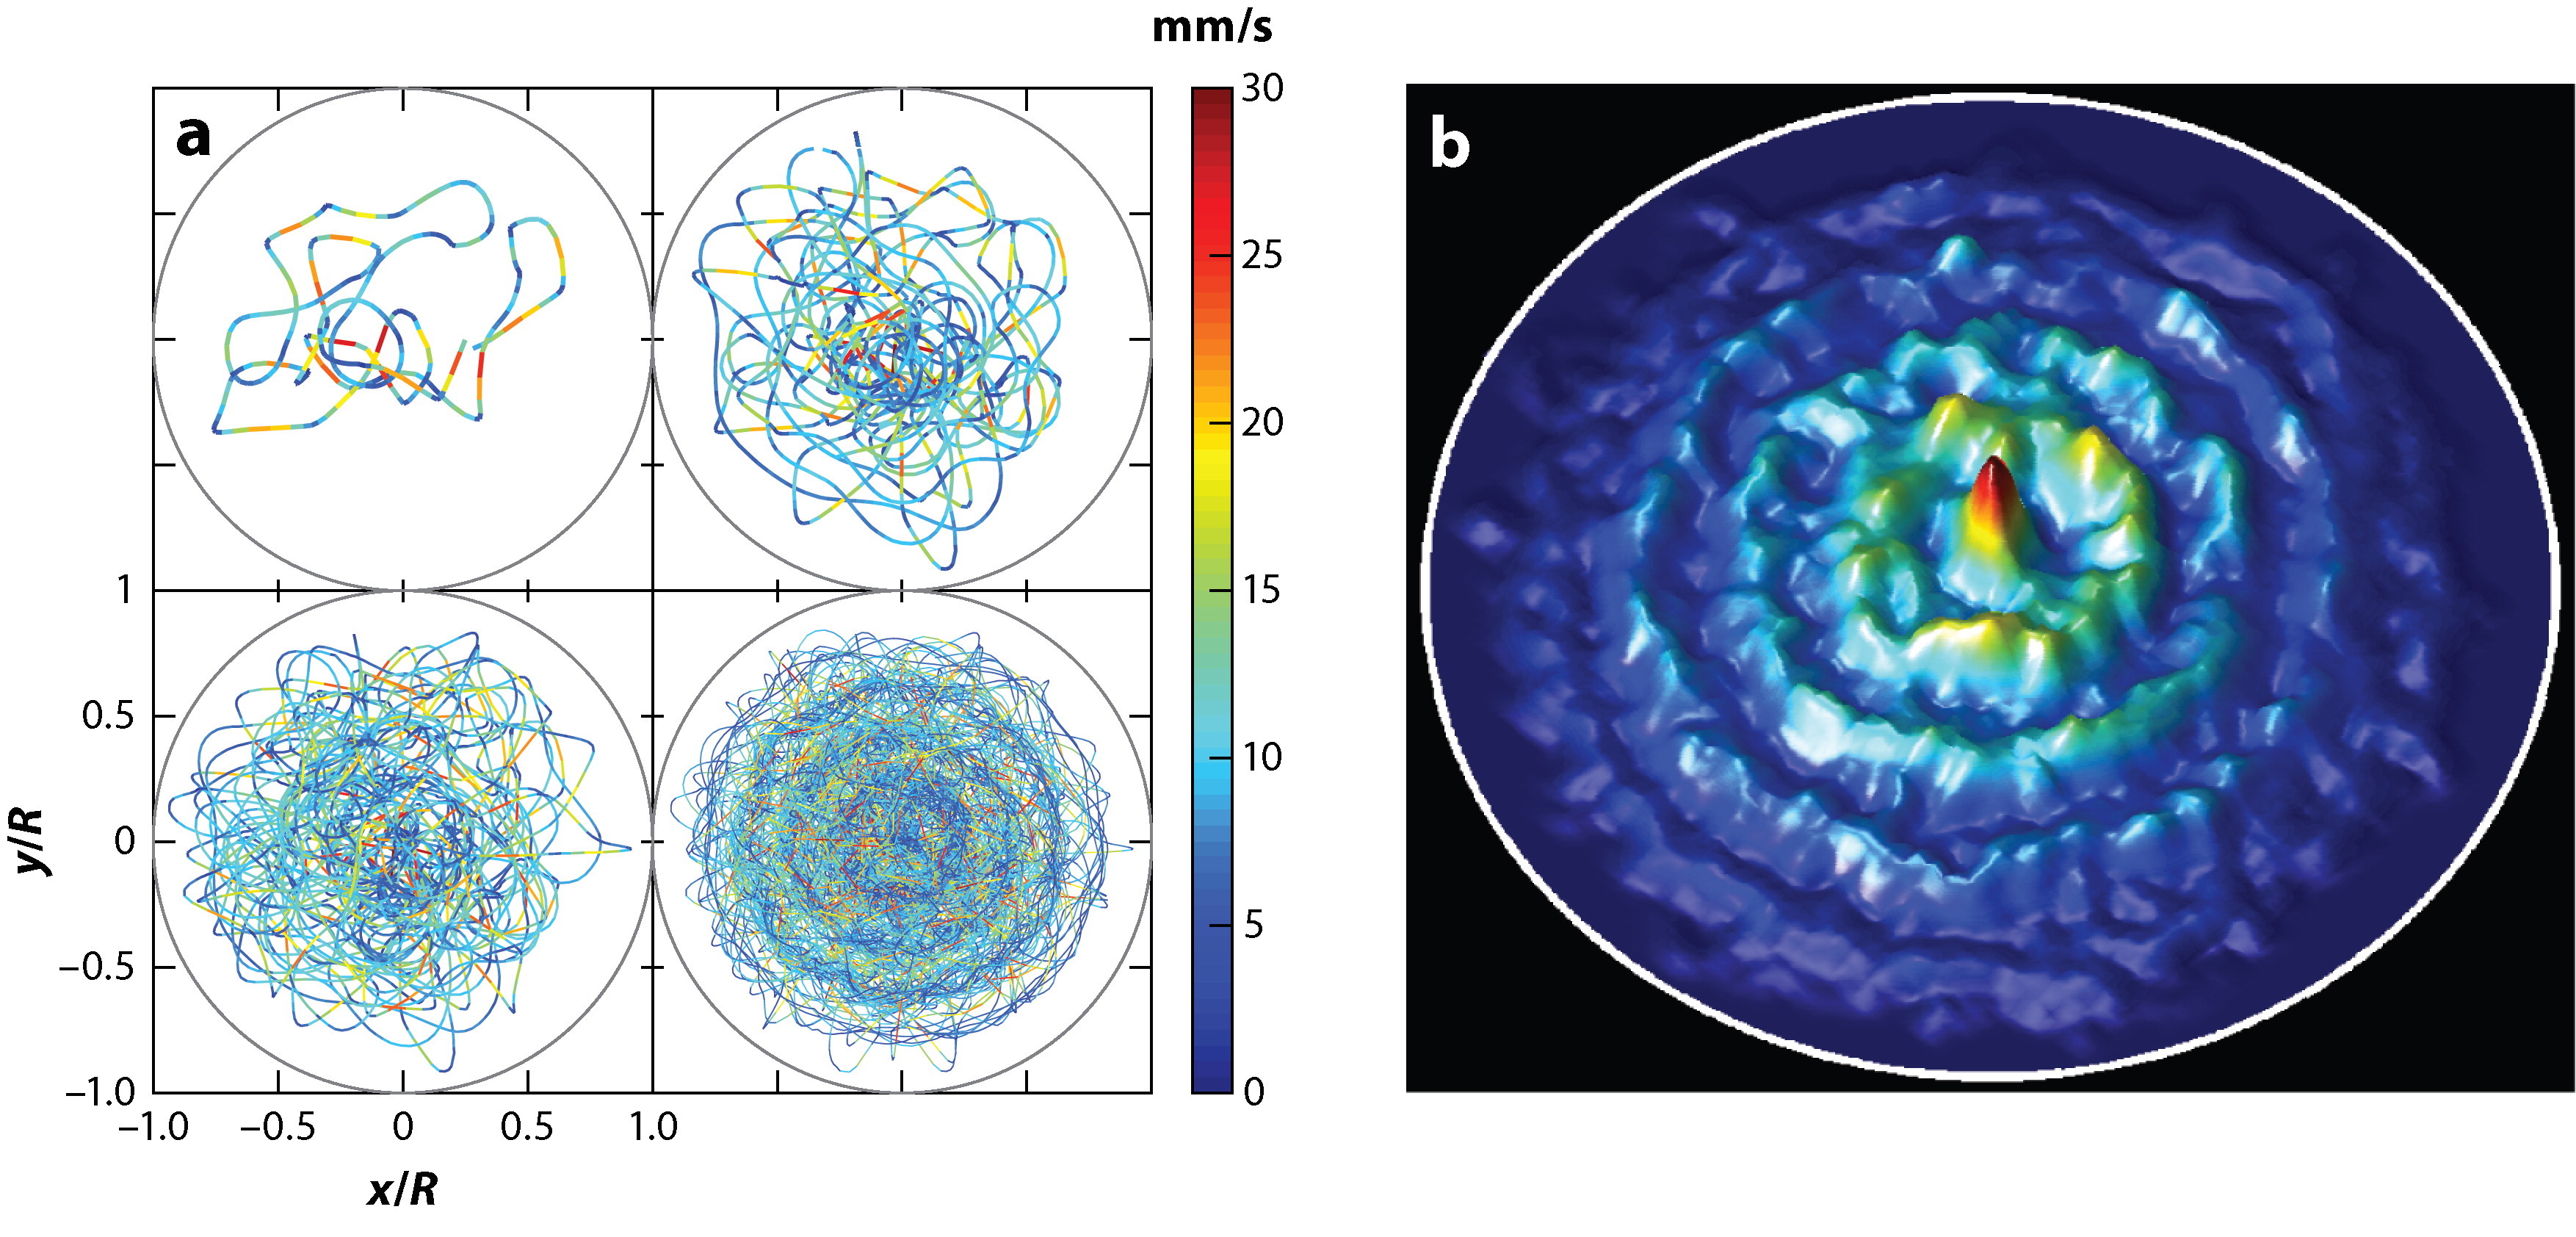
\includegraphics[scale=.115]{stat}
	     \caption{ The figures show the motion of a single chaotic walker in a confined circular geometry. In (a) the path of the moving droplet is traced, where color indicates the velocity of the droplet. In (b) a histogram shows the droplet's position within the circular corral over a span of time. A clear pattern emerges: the droplet appears to be contained within a statistical wave of wavelength $\lambda_\mathrm{F}$. Adapted from J. W. M. Bush, Annu. Rev. Fluid Mech. \textbf{47}, 275 (2015).
	     }
	 \label{stat}
	\end{figure}



\subsection{Tunneling}
\label{sect:tunneling}

    \subsubsection{Tunneling in Quantum Mechanics}
    
Among the various phenomena associated with quantum mechanics, tunneling is one of the most surprising. At the classical level, we can take the example of a basketball thrown at a brick wall: the ball will hit the wall and bounce back every time we try it. When we shift to the quantum scale, if we have a particle headed towards a barrier of a given potential energy, it will not necessarily bounce back. Depending on the characteristics of this potential, there will be a few times in which the particle will \textbf{tunnel} through the barrier, shooting out on the other side. It is not completely fair to use the basketball/wall example as an analogy for the particle/barrier interaction because the ``effective potential energy" of the brick wall is almost infinite, while that of the quantum potential barrier that allows tunneling, is not. For a high enough potential, the particle will also (almost) always bounce back. The point is that probabilistic tunneling cannot be seen at a classical scale in the way that is at the quantum scale, at least not until the discovery of the bouncing droplet system.

    \subsubsection{Tunneling in the Bouncing Droplet System}

\begin{figure}[h!]
 \centering
	    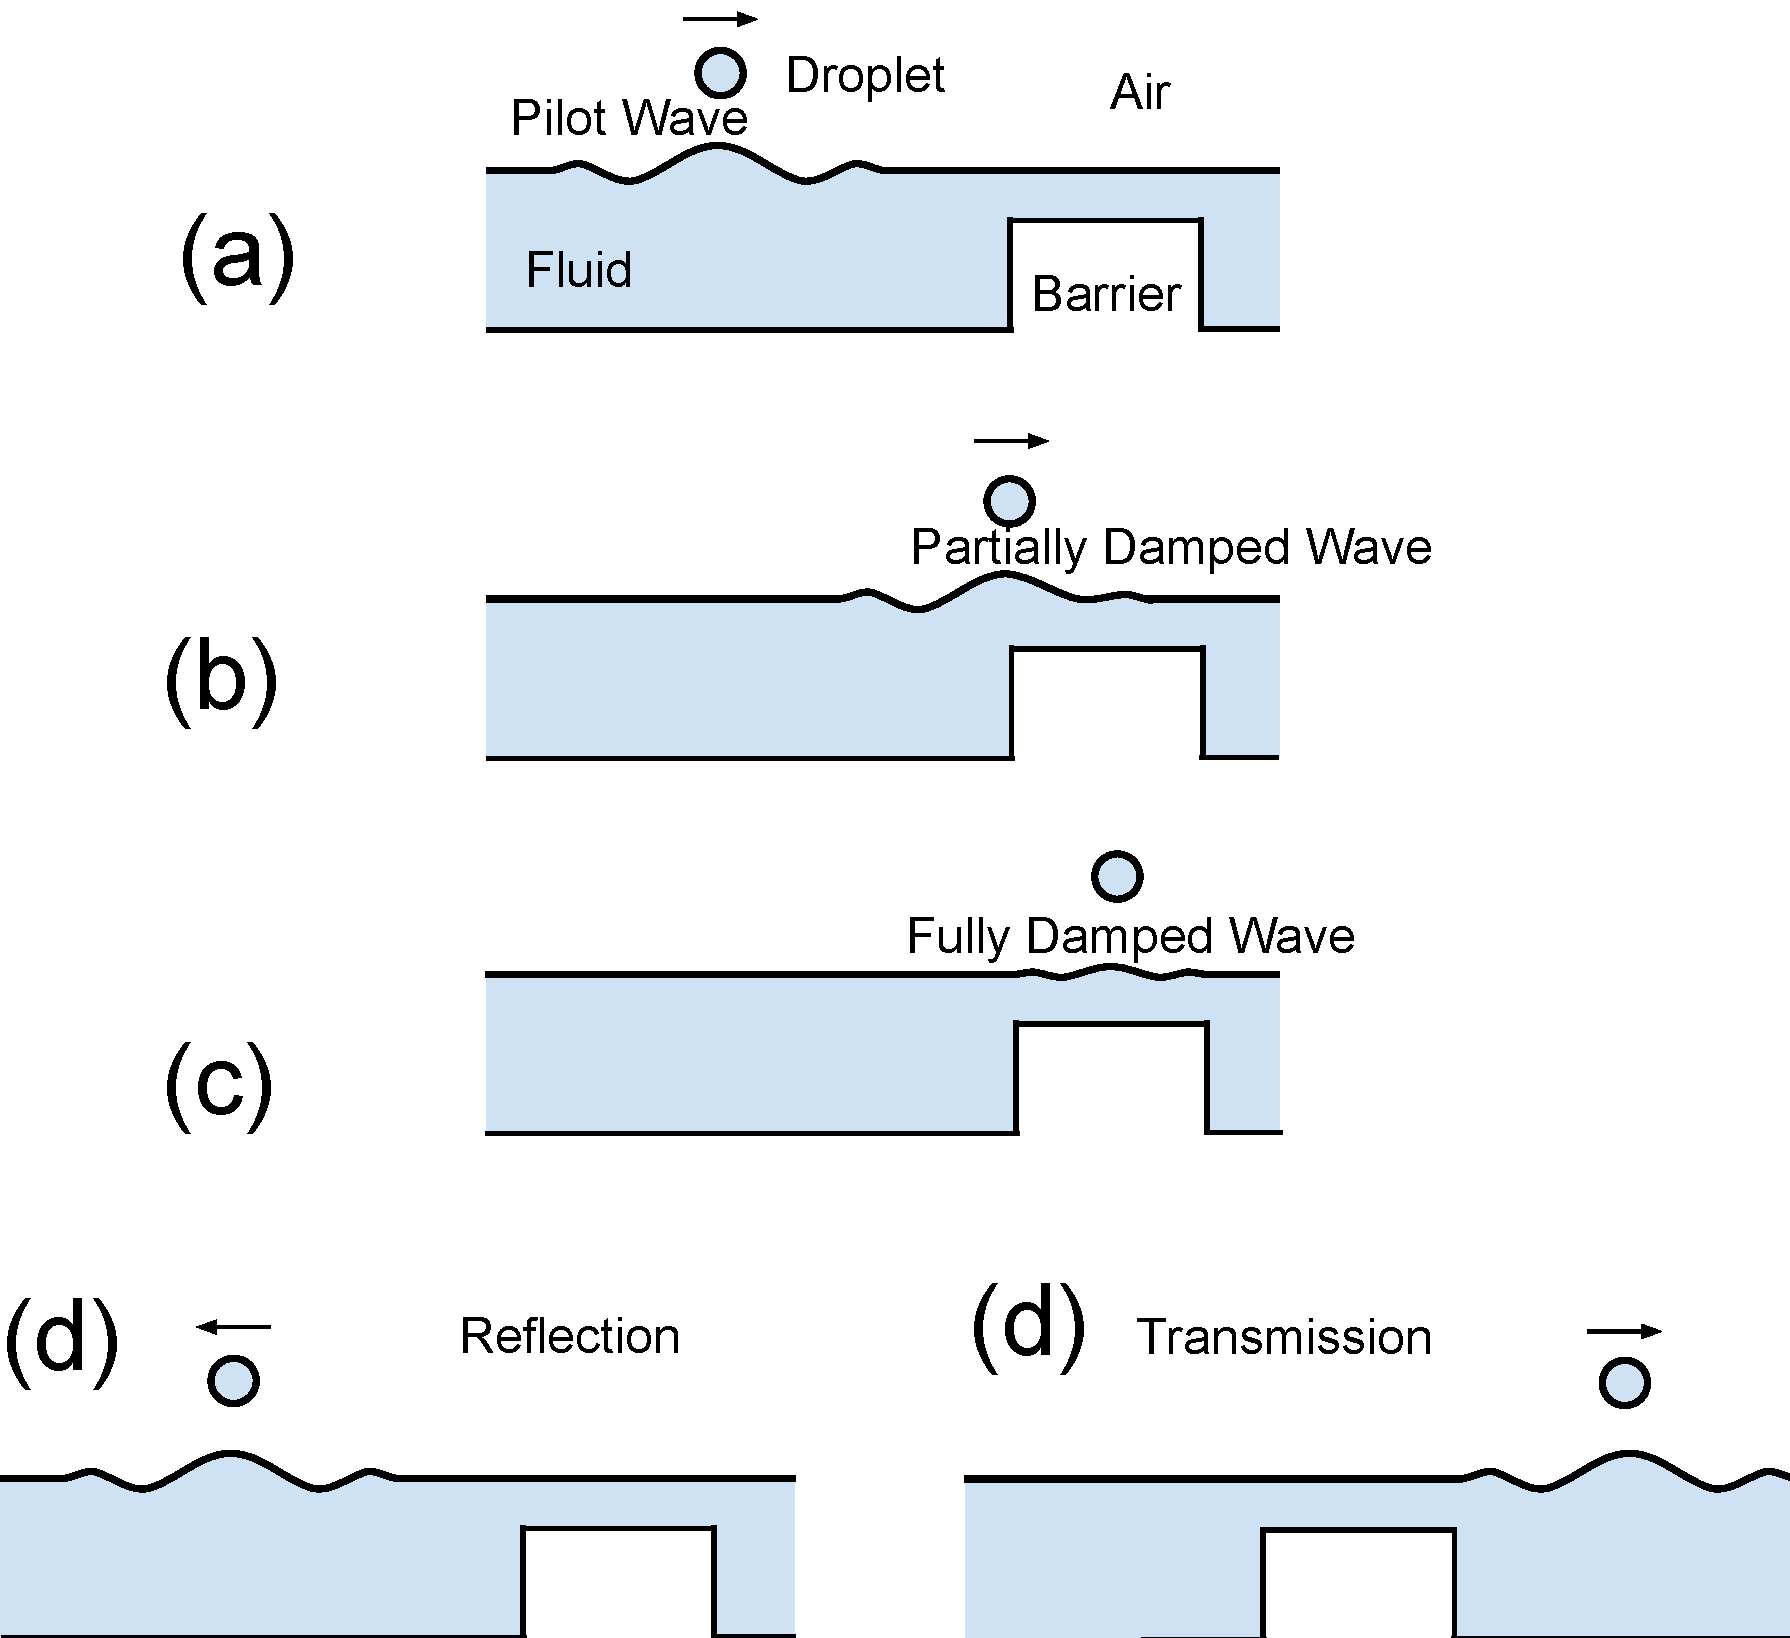
\includegraphics[scale=0.5]{Tunneling}
	     \caption{A diagram of the droplet-barrier interaction. In (a) the walker moves towards the barrier. As it gets closer (b), the guiding wave is damped. In (c) the guiding wave is fully damped such that the droplet is no longer a walker but a bouncer. Guided by the waves the droplet generated as a walker, the bouncer will either be reflected back from where it came (d), or carry on as shown in (e).}
	 \label{tuncartoon}
	\end{figure}
	A study performed by Eddi et al. examined tunneling in the bouncing droplet system \cite{tunneling}. In this setting, tunneling takes the form of the droplet tunneling through (or being reflected by) a submerged barrier. The droplet never actually travels through the barrier, since it bounces on the interface, but the analog to quantum tunneling remains because as the droplet approaches the barrier it is affected by the region of a different ``potential". 
	
For a different depth of fluid $H$, a tray will have a different $\gamma_\mathrm{W}$. If a tray has various regions of different depths, then these different regions will behave slightly differently. This means that when a walker travels from an area of one depth to an area of another depth, its behavior may change. This effect can be seen when a walker is pushed back from a submerged step, seemingly without any contact with the droplet. However, in certain cases, the walker will actually ``tunnel" across the step; that is, it will continue to walk along the surface of the oil bath and pass into the new region of different depth, without reflection. Adjusting the width of the barrier as well as its height will affect the behavior of the droplet. If we make the barrier of width $e$ with height such that the depth of the oil above it is $h$, in a bath that otherwise has depth $H$, then we can think of it as a potential barrier. The unpredictability of the tunneling comes from the complex interaction between the drop and its guiding wave. 

Now say we set $\gamma$ such that walking occurs in the deeper section, but not in the more shallow section (i.e.  $\gamma_\mathrm{W}(H)<\gamma<\gamma_\mathrm{W}(h)$). Then, the droplet is simply a bouncer when in the shallow region, but a walker everywhere else. If the droplet starts out in the deeper region but crosses over to the shallow barrier, it slows down since it is no longer generating the self-propelling waves required for the walking motion. Instead, the superposition of previous waves is what guides it either through or away from the barrier. However, if a droplet were to be created on the barrier, it would remain motionless. Therefore, we can understand the act of tunneling proceed as follows: the walker approaches a barrier, crosses the barrier as a bouncer, and eventually returns to the deeper region as a walker. The process is depicted in \refFig{tuncartoon}. 

\begin{figure}[]
  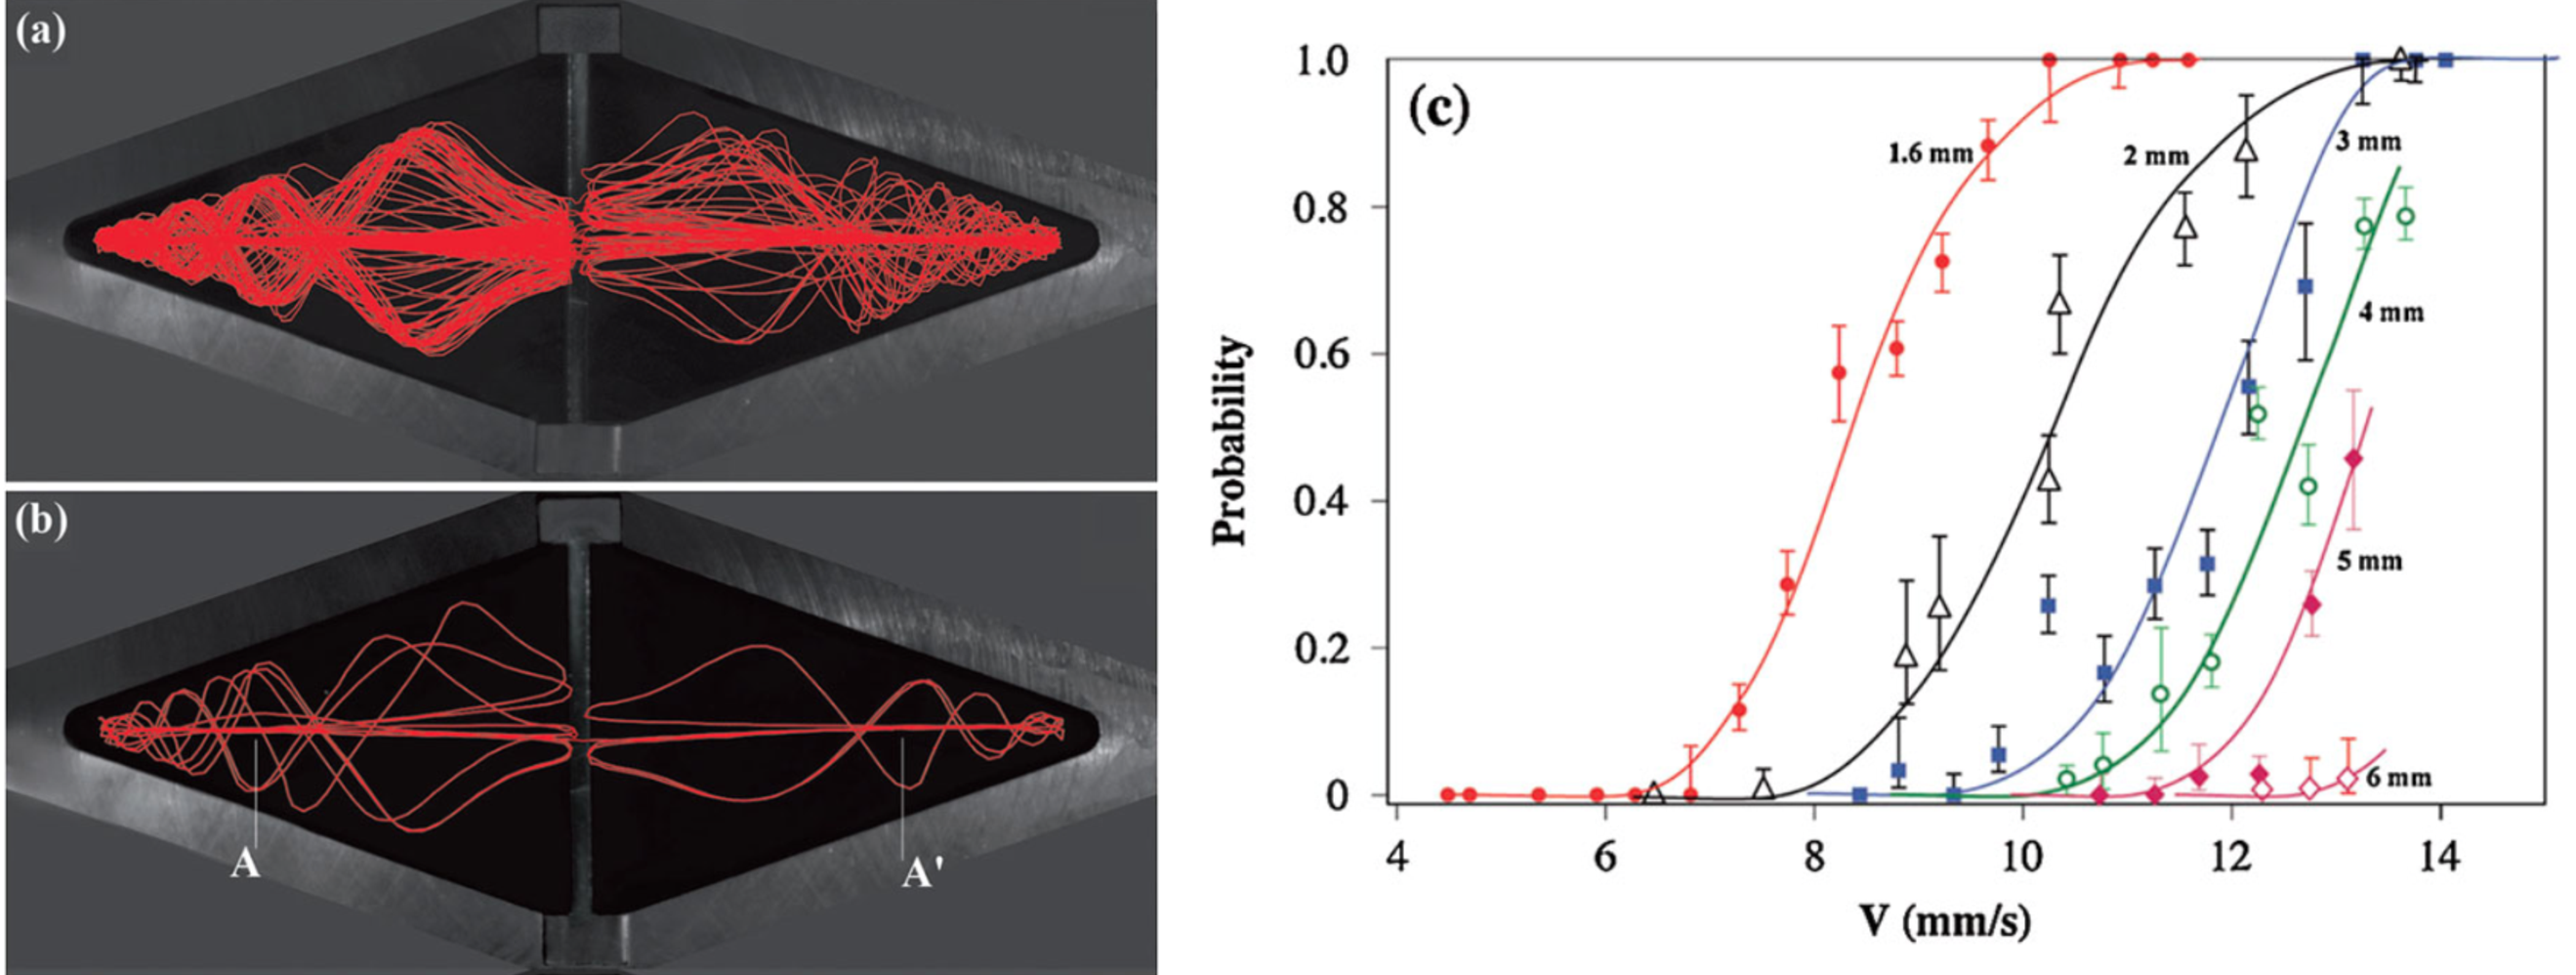
\includegraphics[width=1.0\linewidth]{EddiCombo}
\caption{In (a) and (b) we see the path of a droplet traced out over many collisions with the barrier within rhombus shaped tray. The plot (c) shows the tunneling probability as a function of walker velocity for different barrier widths. Figures adapted from A. Eddi et al., Phys. Rev. Lett. \textbf{102}, 240401 (2009).}
\label{fig:Eddi}
	\end{figure}

Eddi et al. built a tray with a submerged rhombus shape which forced the walker across the center of the tray as shown in \refFig{fig:Eddi} (a) - (b) \rf{tunneling}. A barrier was then placed along the diagonal of the rhombus, perpendicular to the direction of travel of the walker, so that the walker would run directly into the wall. They showed that as $\gamma/\gamma_\mathrm{F}$ approached $1$, faster droplets had higher probabilities of tunneling (\refFig{fig:Eddi} (c)). They also discovered that by increasing the barrier width, the tunneling probability decreased. 

The question that lingers, and that is the focus of this thesis, is the following: \textbf{How does tunneling probability change as a function of oil depth above the barrier \textbf{\textit{h}}?} We expect that at large $h$ values the localized Faraday waves will be less damped, meaning that the walkers will tunnel more frequently. At small values of $h$ where the localized Faraday waves are heavily damped, it is predicted that there will be very little tunneling. What is the critical height where we see both behaviors? An experiment, detailed in the following chapter, was designed to test this question.
    
	%\chapter{Introduction to Tunneling in QM}	


\section{Wavefunction}	
In classical mechanics, one can describe a particle with six variables: three position indicators ($x$, $y$, $z$), and three momentum indicators ($p_x$, $p_y$, $p_z$). One can find a function to represent variable by making multiple measurements across time, and discover an expression $x(t)$ that describes the particles location in space along the x dimension at time $t$. When all six variables can be described by a function, one can describe the position of the particle at any time.  

In quantum mechanics however, Heisenberg's uncertainty priciple limits the knowledge of position and momentum: 
$$\sigma_{x} \sigma_{p} \geq \hbar/2. $$
This equation states that as one knows more about the position of the system, then one loses knowledge about the momentum of the system, and vis versa. It's a tradeoff inherent to the nature of the system, not due to experimental deficiences. And it means that the strategy of finding equations for position and momentum of a system are no longer possible. If a particle has no exact position, can one represent where it might be? One can use a wave describing the probability of finding the particle at that position. The square root of this wave is called the wavefunction, and is represented by $\Psi(x, t)$.


\section{Schroedinger's Equation}

The wavefunction $\Psi(x, t)$ is goverened by the Schroedinger equation:

$$i\hbar\frac{\partial}{\partial t} \Psi(x,t) = \left [ \frac{-\hbar^2}{2m}\frac{\partial^2}{\partial x^2} + V(x,t)\right ] \Psi(x,t) $$
where $V(x,t)$ is the given potential, $m$ is the mass of the particle, and $\hbar$ is the reduced Planck's constant. For potentials that do not change in time, one can use separation of variables to arrive at the time-independant Schroedinger equation
$$E \Psi(x,t) = \left [ \frac{-\hbar^2}{2m}\frac{\partial^2}{\partial x^2} + V(x)\right ] \Psi(x,t)$$
where $E$ is the total energy. The goal is to find $\Psi(x,t)$ knowing the potential $V(x)$.




\section{Barrier Potential}

\section{Energies}
    \subsection{$E = V_0$}
    \subsection{$E > V_0$}
    \subsection{$E < V_0$}
    
    
    
    
\section{Physics}

Many of the symbols you will need can be found on the math page (\url{http://web.reed.edu/cis/help/latex/math.html}) and the Comprehensive \LaTeX\ Symbol Guide (enclosed in this template download).  You may wish to create custom commands for commonly used symbols, phrases or equations, as described in Chapter \ref{commands}.


	\chapter{Experimental Design}

In the our bouncing droplet system we observe surface waves guiding a droplet, and we're interested in learning more about the droplet-wave system in different settings. In this experiment, we will look at how features \textit{underneath} the surface of the oil (i.e. on the ``floor" of the tray) affect the motion of the droplet. 

A raised object on the floor of the tray (but still underneath the surface of the oil) can have an effect on height of the surface waves, and thus, on the motion of the walker. Sometimes a droplet headed towards a raised object will be reflected backwards, as if from a collision with the object. For this reason, we refer to a raised object as a barrier. Oftentimes however, the droplet continues on and crosses the barrier without a collision, this is analagous to ``transmission" the quantum mechanical process of tunneling. In other words, for a given barrier we will see a probability of tunneling unique to that barrier. Other studies have shown that increasing barrier width decreases probability of tunneling\rf{tunneling}. This study looks at how height of the barrier affects the tunneling probability. 

To test the effect of a barrier's height on the probability of tunneling, I used a combination of procedures from the investigations of Bush\rf{pilot-wave}, Couder\rf{Couder2005}, and specifically, Eddi et al.\rf{tunneling}. These were slightly modified to fit some of the unique features of my experiment. In this section I aim to give some of the reasoning behind the tray design and data collection techniques, both of which are not well described in the literature.

\section{Setup}
    The combined setup is shown in \refFig{setup}. A waveform generator creates a sinusoidal signal which is amplified and fed into a shaker. The shaker vibrates the tray vertically. Both the frequency and the amplitude of the vertical oscillations can be controlled. 
    
    An accelerometer records the vertical acceleration of the tray and is read by an oscilloscope. A camera records the droplet as it bounces along the surface of the oil.  
    
\begin{figure}[h!]
	\centering
	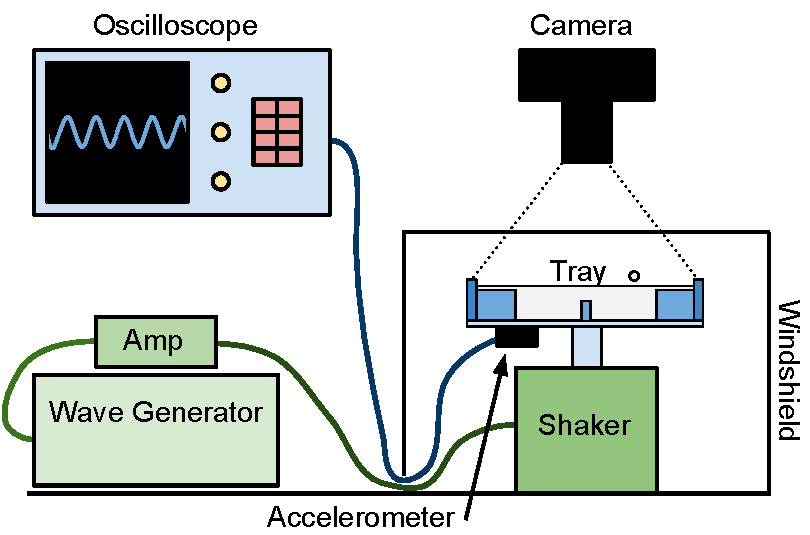
\includegraphics[scale=0.8]{Setup.pdf}
	\caption{The experimental setup. The amplified signal from the wave generator drives the shaker. The accelerometer generates a signal which is read by the oscilloscope. The shield blocks disturbances to the experiment, while allowing the camera to document the trials.}
	\label{setup}
\end{figure}

\section{Materials}
The key components of this experiment are the shaker, the oil, and the tray. In this section I'll describe the specifics of the holy trinity, as well as some of the additional components used in data collection. 

\subsection{Tray}
The tray was made of plastic parts machined by the (MODEL NUMBER?) laser cutter. They were then glued together with GLUE?. The tray's design, which was based off of the tray in the tunneling experiment done by Eddi et al.\rf{tunneling}, naturally guides the droplet into a perpendicular collision with the barrier. The tray schematic is shown in \refFig{tray}. 

\begin{figure}[h!]
	\centering
	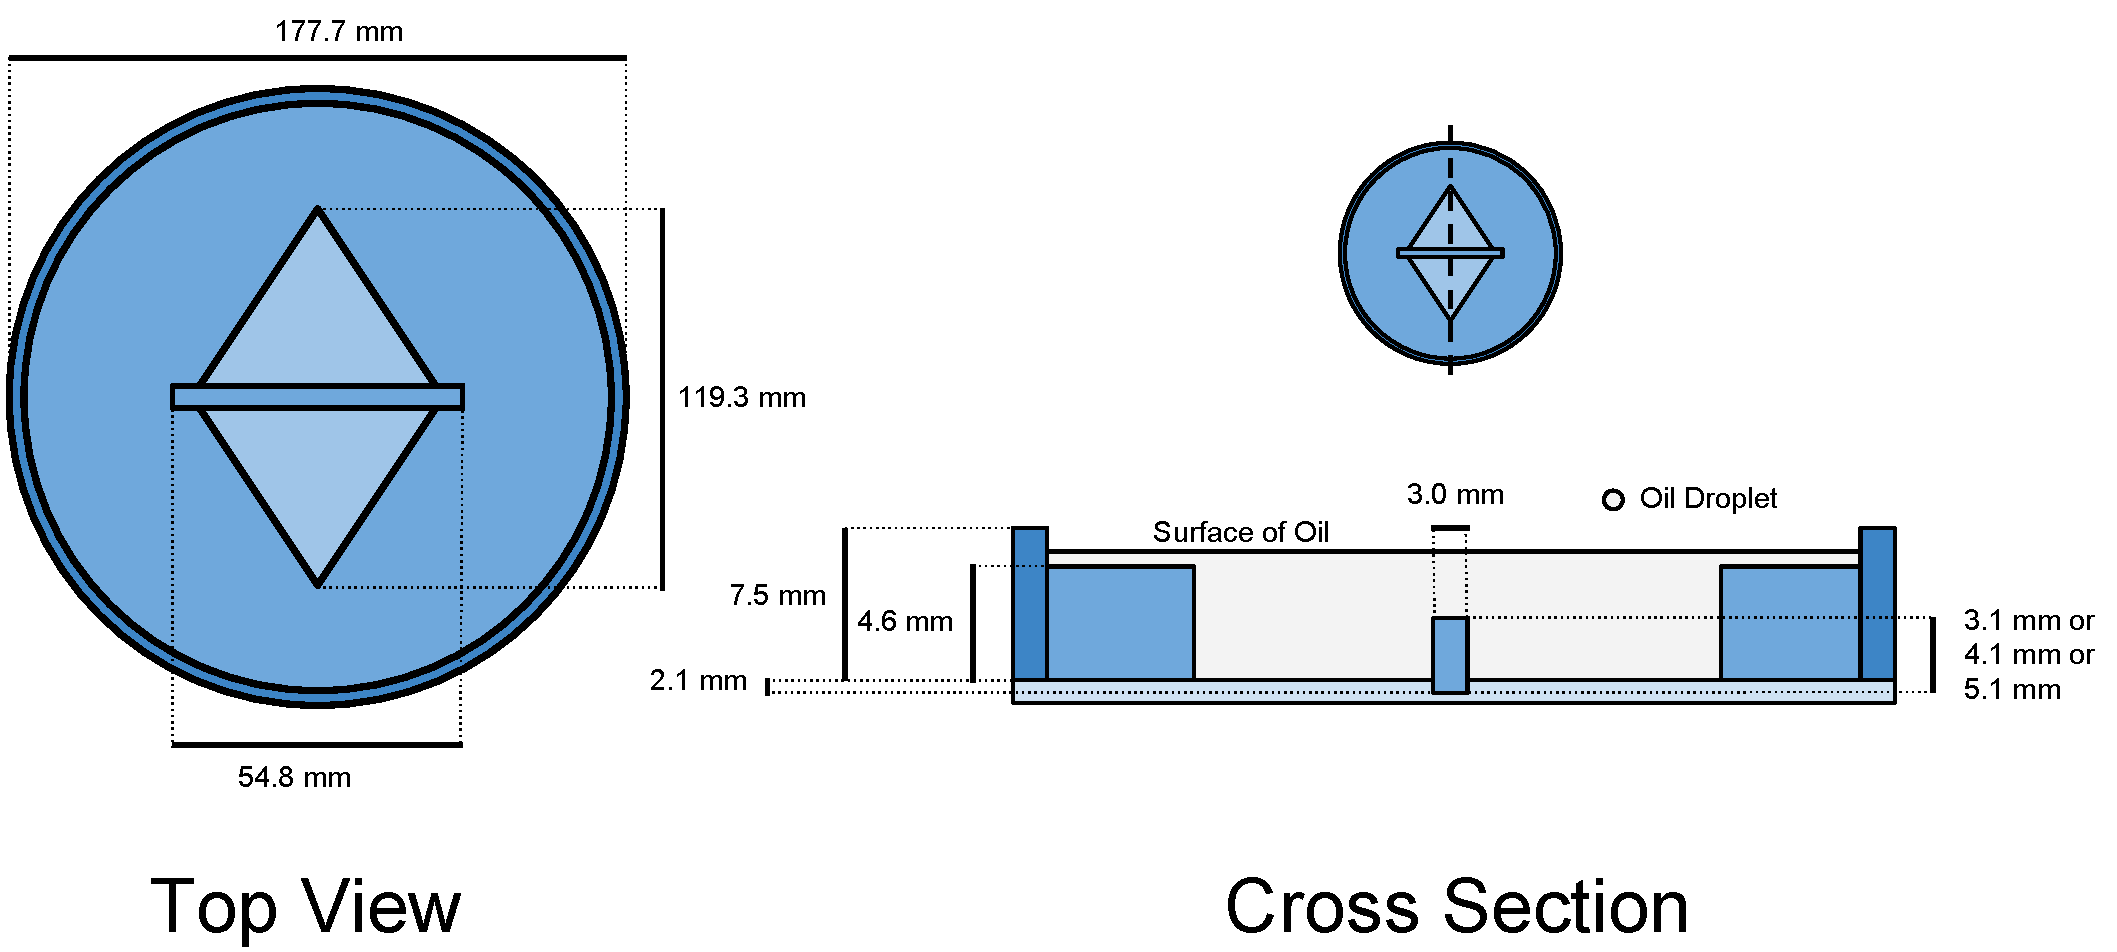
\includegraphics[scale=0.48]{Tray.pdf}
	\caption{The specifications of the tray design. The top view (left) highlights the main elements in the tray, while the cross section (right) illustrates the topography of the tray. Height is represented by the shading; darker shading is higher.}
	\label{tray}
\end{figure}

A thin layer of oil spills over the constraining rhombus shape. As long as the layer is thin enough, the droplet will remain in the rhombus container, but the waves will continue to propagate unimpeded. This gives the waves time to decay, and means that the droplets motion isn't chaotically affected by reflections of previous waves from the sidewalls, and is instead guided only by the unreflected waves. 

The rhombus shape serves to steer the droplet into a perpendicular collision with the barrier. This works because the droplet will pin-ball its way into the acute corner of the rhombus, and will shoot out in a straight line, directly towards the barrier.  (FIGURE of pinballing droplet?)

I designed my experiment to test barriers of three different heights: $2.75~\mathrm{mm}$, $3.0~\mathrm{mm}$, and $3.25~\mathrm{mm}$, measured from the bottom of the rhombus. A thin barrier of plastic made by the laser cutter has the tendency to bend and warp over time. The solution to this problem was to make these barriers taller than the specified heights, and create an cut-out in the rhombus so they could be inserted. The barrier cut-outs were deep enough to exactly counter the added height of the barrier, so the barriers still had (when measured from the surface of the rhombus) heights of $2.75~\mathrm{mm}$, $3.0~\mathrm{mm}$, and $3.25~\mathrm{mm}$. This also solved the problem of fixing the barriers in place, but still making them easily removable. These heights were chosen because they allowed for both passage over and blockage by the barriers. At the lowest heights, most droplets crossed over, whereas for taller barriers most droplets were blocked. 


The bottom of the tray was painted black in order to improve contrast, allowing the droplet to be more easily tracked by eye and by camera.

\subsection{Silicon Oil}
    Silicon oil is the ideal choice of fluid for this experiment because it remains clean, it doesn't evaporate, and it can be purchased at specific viscosities. The silicone oil used in this experiment had a viscosity of 20 cSt (its viscosity is a little closer to water than olive oil) and was purchased from Clearco Products Co. Inc., Bensalem PA (CAS No: 63148-62-9). 20 cSt silicone oil, like the one used by Bush et al.\rf{pilot-wave} was chosen because it gives a larger walking regime\rf{pilot-wave} than more viscous oil, such as the 50 cSt viscosity oil used by Couder\rf{Protiere2005}. The tray requires about $20~\mathrm{mL}$ of fluid.
    
    It is of vital importance to keep the oil as clean as possible because it keeps the droplet bouncing for longer. This means protecting from particulate matter that is already in the tray. Contamination can be minimized by cleaning the tray before pouring the oil in.
    
\subsection{Shaker}
    To shake the tray, we used a mechanical wave driver made by Pasco Scientific, Roseville CA, model SF-9324. This shaker was designed to drive a string or an elastic cord, not a $200$ gram tray with oil inside, which was probably at the limit of what the shaker can handle. 

\subsection{Waveform Generator and Amplifier}
    The shaker was driven with the Agilent Arbitrary Waveform Generator model 33210, which was controlled digitally and thus created consistent waves.  
       
    Adding a Lepai LP2020A+ digital amplifier to the wavefunction generator meant the amplitude of the tray could be precisely controlled. This signal was then fed into the shaker.    
            
\subsection{Accelerometer}  
    Knowing the tray's acceleration allows us to characterize the behavior of our system. To measure acceleration, we attached an ADLX 326 triple axis accelerometer (made by Adafruit, New York City NY) to the bottom of the tray. The method of attachment was screws, since it provided a much more firm hold than tape or glue while allowing for removal. The accelerometer has a range of $\pm$16$g$, perfect for measuring the accelerations in our setup, usually below $5g$'s. 
      
      The signal from the z-axis of the accelerometer was output directly into the oscilloscope. For the vibrating tray, the output was approximately sinusoidal (as expected). The spec sheet for the accelerometer indicates that the sensitivity can be translated to $57 \pm 6~\mathrm{mV/g}$. 
 
    
\subsection{Shield}
    A large, see-through cylinder (covered at one end) was manufactured using the laser cutter. When placed over the tray, it served the purpose of keeping the oil clean from particulate matter and preventing wind currents from influencing the motion of the walker.       
   
\subsection{Leveling Platform}
    A leveling platform was made out of wood supports the shaker. Three adjusters allowed for precise adjustment of tilt. The tray was tuned using a level placed inside the tray (before the oil was added). 

\subsection{Camera}       
 
To document trials, a Sony RX100 camera supported by a tripod aimed directly down at the tray. 

\section{Procedure}
Once the exact walking parameters are established (frequency and driving amplitude), tunneling measurements and a few different barrier heights can be made. 

\subsection{Finding the Walking Regime}

Before investigating the rate of tunneling using different barriers, a rough estimate of the walking regime at a frequency of $80~\mathrm{Hz}$ must be made. A ``map" similar to the one in \refFig{regime} will be sketched out, but rather than looking at all of the different kinds of bouncing we will limit ourselves to only the walking regime. Reproducing this figure allows us to find the parameters that are specific to our unique setup, which could have slightly different height, tray, oil, and shaker configurations than those used in the literature. 

Droplet size is measured using a recorded video of the walking droplet in motion. By comparing the number of pixels making up the diameter of the droplet (unknown measurement) to the number of pixels making up the diameter of the tray (known measurement), we can estimate the length associated with  each pixel, and thus find the diameter of the droplet in centimeters. 

Driving acceleration values are measured by the accelerometer and displayed on the oscilloscope. 

To ensure that every trial has the same oil depth, we must measure the volume of the oil before filling the tray. Knowing the volume of the tray and of each barrier, we can get a value for the oil depth without interfering with the system. In this way, oil height can be kept constant.

\subsection{The Experiment}

Tunneling was examined for three different barrier heights. At each height (and at a constant frequency of 80 Hz and constant driving acceleration), a string of continuous collisions were filmed with the camera. From this data, a basic tunneling probability was calculated, which provides the most simplistic analysis of this system. 

The tray is designed such that most of the droplet's collisions with the barrier occur ``head on" (i.e. perpendicular to the length of the barrier), but not all collisions unfold ideally. A more involved analysis in \textit{Tracker} requires looking at the component of velocity of the droplet perpendicular to the length of the barrier, and determining the probability of tunneling given this value. Since not all collisions in the simplistic analysis occur at the same velocity, this method allows for a more methodical analysis of the phenomena. 

	
	\chapter{Data Analysis and Results}

In this chapter, I will summarize the raw data that I collected and the findings I generated. A closing discussion on the sources of error keeps us grounded.

%-------------------------
%        RAW DATA
%-------------------------
\section{Raw Data}
The raw data consisted of a total of 7 videos and are laid out in \refFig{datacollection}. Barrier height, acceleration of the tray, Faraday threshold, and percentage of ``transmissions" were recorded for each of the 7 videos. The 7 videos contained: one trial of a single droplet for all three barrier heights, another trial of a single droplet for all three barrier heights, and a final trial of a single droplet for the $3.0~\mathrm{mm}$ barrier. By switching the barriers while the tray was still shaking we were able to use same droplet for each of the three barrier heights in a trial. There were between 12 to 24 separate collisions for each barrier. 

\begin{figure}[h!]
	\centering
	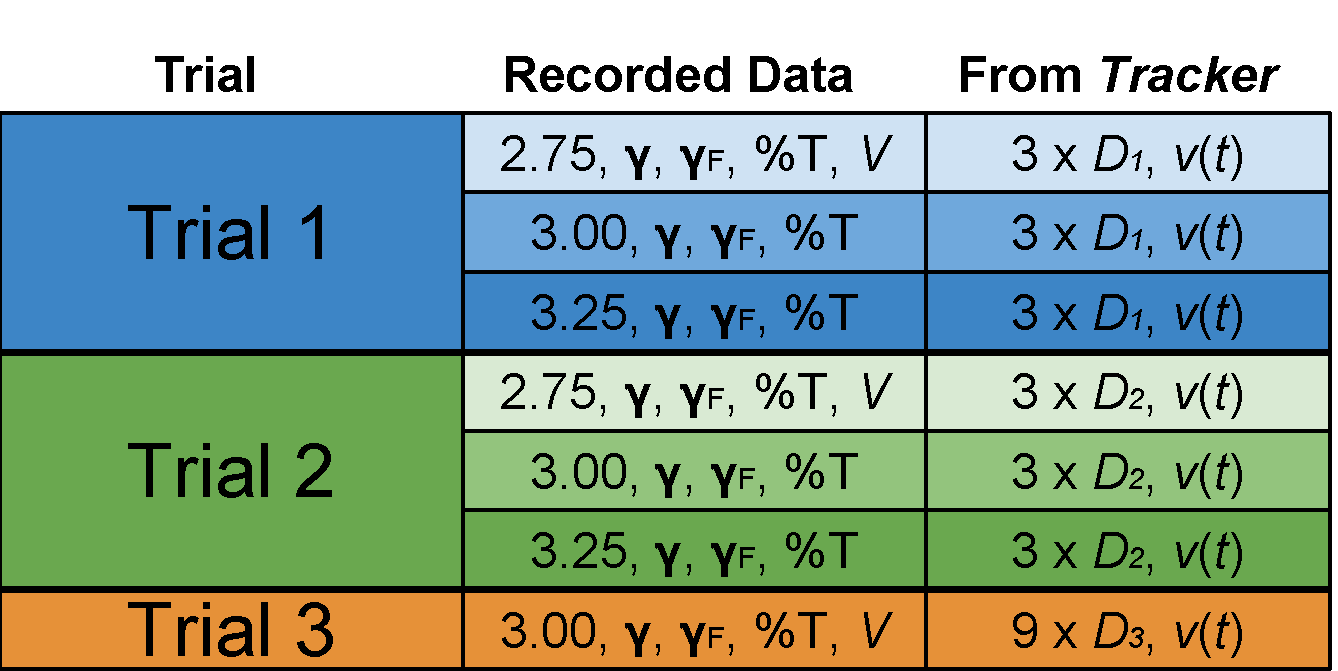
\includegraphics[scale=0.4]{datacollection.pdf}
	\caption{For each barrier ($2.75~\mathrm{mm}$, $3.0~\mathrm{mm}$, or $3.25~\mathrm{mm}$), the forcing acceleration $\gamma$, the Faraday threshold acceleration $\gamma_\mathrm{F}$, and the percentage of ``transmissions" (\%T) were recorded. The oil volume $V$ was recorded at the beginning of each trial. From \textit{Tracker}, measurements of the droplet diameter $D_n$ in three randomly selected frames were made, along with the velocity of the droplet for every frame $v(t)$.}
	\label{datacollection}
\end{figure}

These movies were then processed with \textit{Tracker} \cite{tracker}. \textit{Tracker} decomposes a video into multiple frames for the purpose of tracking an object in a video. The Autotracker function marks the position of the object in every frame and records the time in between each frame ($\frac{1}{24}$ seconds), and using this information \textit{Tracker} estimates the velocity of the droplet at every frame. We also want to know the size of each droplet, so we measure the diameter of the droplet using a function in \textit{Tracker}. The diameter is measured 3 times in each movie, yielding 9 total measurements per trial. These nine measurements were averaged to estimate the diameter of the droplet used in that trial. In trial 3, where only one barrier was used, 9 independent measurements were made, as detailed in \refSect{sect:error}.

From the volume of the oil $V$ measured with a graduated cylinder, and measurements taken of the tray, we can calculate the parameter $h$, which is defined as the height of the oil above the barrier. This was done by calculating the volume the ``space" inside the tray, which required accurate dimensions of the tray. %\footnote{The function making this calculation can be found in the Appendix.}

Values for the various parameters in this experiment are shown in \reftab{explimits}. Error estimates are discussed in \refSect{sect:error}.

	       \begin{table}[htdp] 
\caption[Basic Table 1]{Values of the various parameters in this experiment.} 
\begin{center} 
\begin{tabular}{c c} 
\toprule 
  Parameter &  Lower Limit\\
  \midrule
Viscosity $\nu$ (cSt) & 20.0 \\ 
Frequency $f$ (Hz) & 80.0 \\
Memory $\gamma/\gamma_\mathrm{F}$ & $0.983 \pm 0.003 $ \\
Drop Diameter $D$ (mm) & $0.99$ to $1.07 \pm 0.04$ \\
Bath Depth $H$ (mm) & $4.26 \pm 0.35$ \\
Oil Depth Above Barrier $h$ (mm) & $0.99$ to $1.52 \pm 0.35$ \\ 
\bottomrule 
\end{tabular}
\end{center}
\label{explimits} 
\end{table}	


%-------------------------
%        ANALYSIS
%-------------------------
\section{Analysis}


    \subsection{Tunneling vs. Oil Depth}
The primary purpose of this investigation was to determine how the depth of oil affected tunneling. The results are shown in \refFig{tbh}, indicating that droplet never crossed near the value $h~=~1.0~\mathrm{mm}$, whereas it always crossed at a value $h~=~1.5~\mathrm{mm}$. In between, at a depth $h~=~1.25~\mathrm{mm}$, we have both transmissions and reflections at a rate that changes for every trial. If we consider the droplet diameter, we see that the plot suggests that the transmission coefficient increases depending on the diameter of the droplet. 

The vertical error bars indicate standard error, and the horizontal error bars indicate unceritainty. 

\begin{figure}[h!]
	\centering
	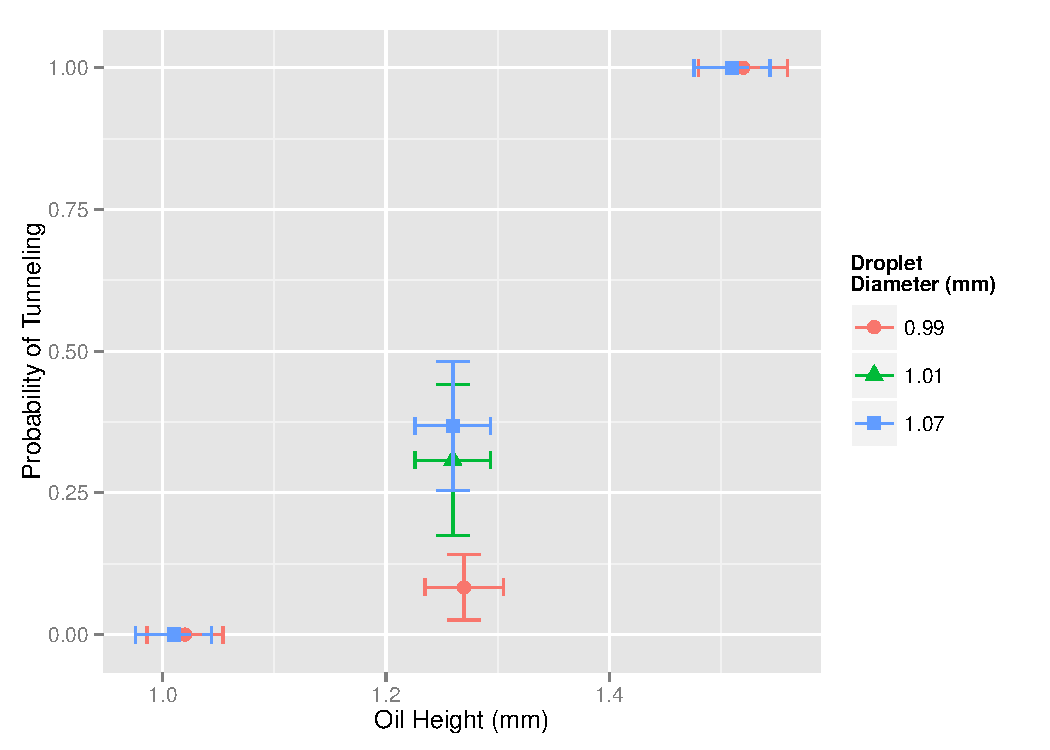
\includegraphics[scale=.9]{TunnelingProb.pdf}
	\caption{The proportion of transmissions for all collisions as a function of oil height above the barrier. Each shape corresponds to a single trial for which the droplet was kept constant.}
	\label{tbh}
\end{figure}


    \subsection{Tunneling by Droplet Velocity}
Not every droplet barrier collision was ideal. Many times, the droplets approached at an angle or at different velocities which means that it is a little misleading to speak as if every collision was exactly the same. One way we can standardize collisions is by looking at the velocity perpendicular to the barrier at $5~\mathrm{mm}$ away from the center of the barrier, as shown in \refFig{tvd}.

\begin{figure}[h!]
	\centering
	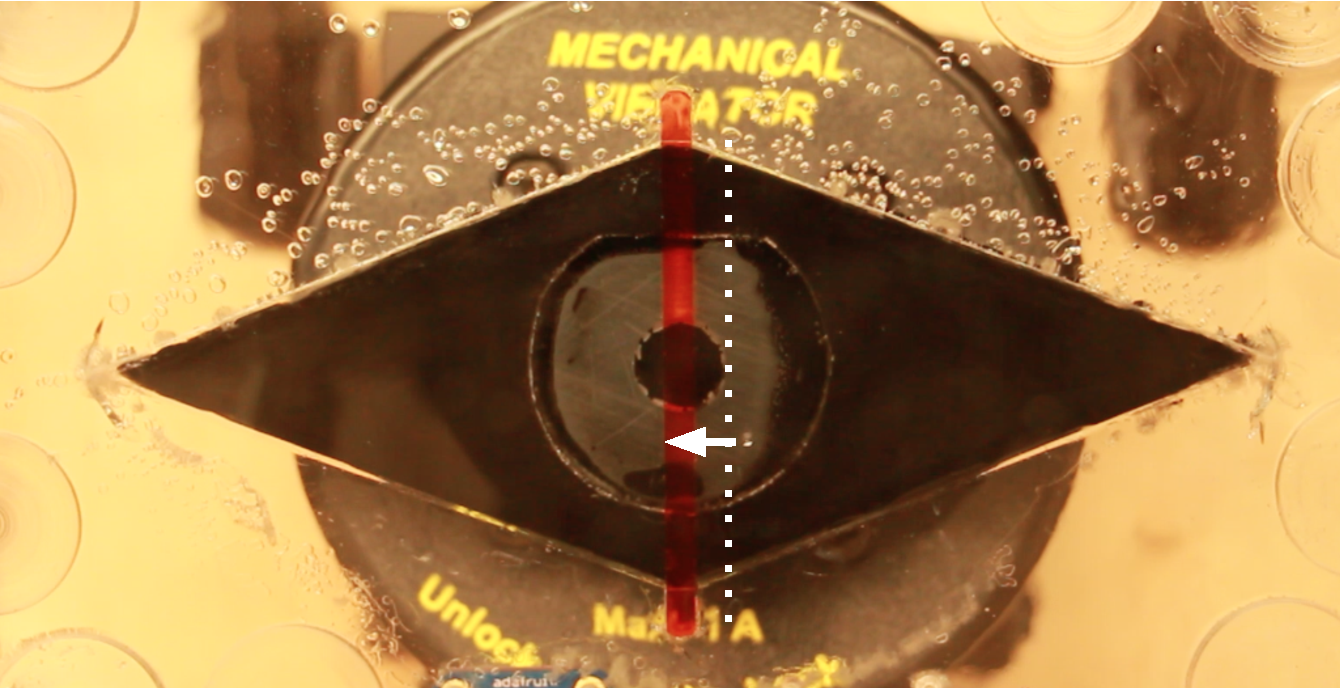
\includegraphics[scale=0.6]{TunnelingVDiagram.pdf}
	\caption{The image shows the point at which the perpendicular component of velocity was made, at $5~\mathrm{mm}$ from the middle of the barrier.}
	\label{tvd}
\end{figure}

We expect the perpendicular component of velocity to be important because it proved critical in the study of barrier width carried out in \rf{tunneling}, and because its intuitive: if the droplet moves faster, it has greater momentum and is more difficult to stop. \refFig{vel} shows every collision for the middle barrier height, and the result of each interaction. In trials 2 and 3, the majority of the droplets with the fastest perpendicular velocities are usually the ones that pass through the barrier, as expected. This does not seem to be the case for trial 1, for unknown reasons. 

\begin{figure}[h!]
	\centering
	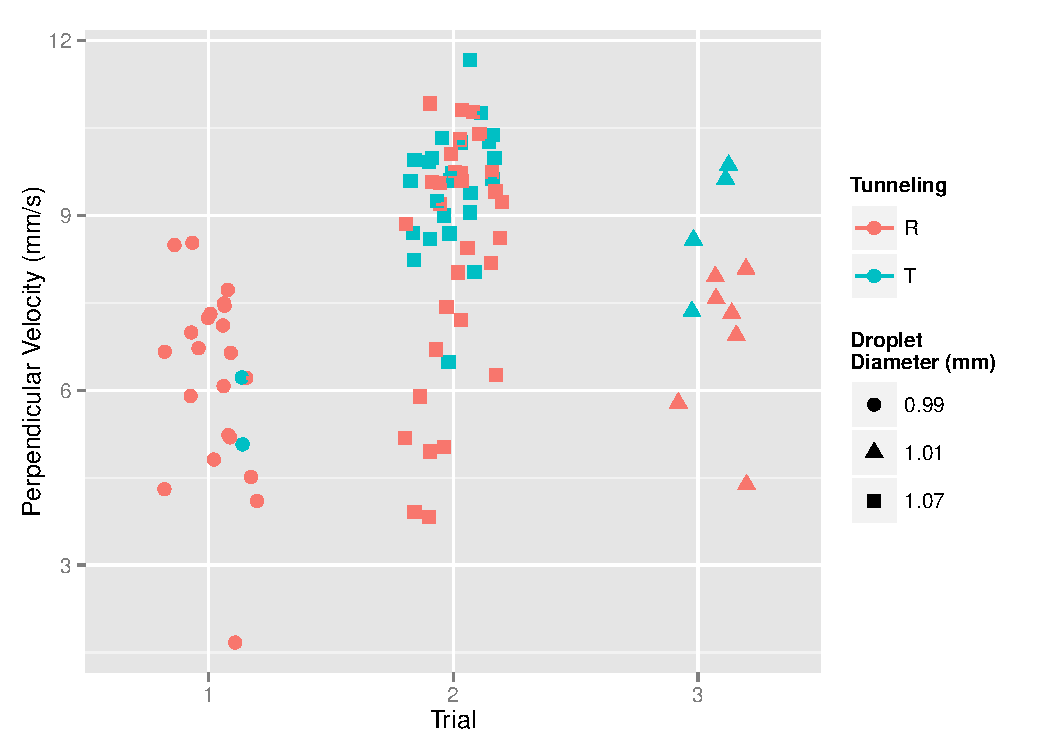
\includegraphics[scale=0.9]{Velocity2.pdf}
	\caption{The result of each collision for the middle oil depth. The color represents the outcome of the collision (either transmission (T) or reflection (R)), and the shape represents the diameter of the droplet. The horizontal spread within each trial was added to aid in visualization.}
	\label{vel}
\end{figure}

Next we try breaking up the collisions by velocity. The collisions from the $3.0~\mathrm{mm}$ barrier were grouped into bins of width $2~mathrm{mm/s}$ and plotted by the fraction of all collisions that tunneled. The result, shown in \refFig{VP}, leaves a little to be desired. We see immediately the major limitation is the lack of trials, and perhaps, in consistency. Trial 3 is the only one that shows the expected trend: as velocity increases so does tunneling. Trials 1 and 2 show valiant efforts that eventually run into the ground. 


\begin{figure}[h!]
	\centering
	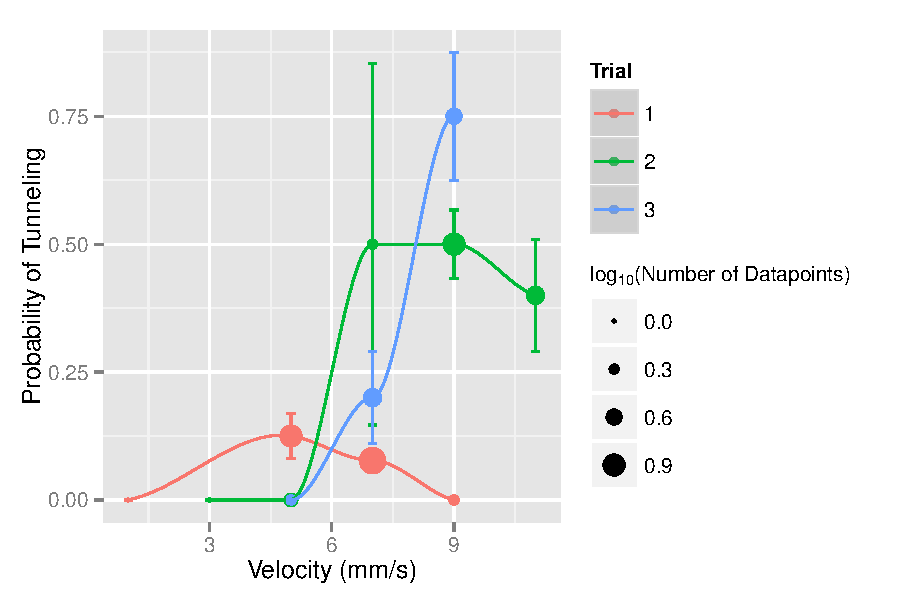
\includegraphics[scale=0.9]{VP.pdf}
	\caption{Collisions of similar velocities were grouped into bins of width $2~\mathrm{mm/s}$. The overall fraction of transmissions was computed for each bin, and plotted. Colors distinguish between trials, and sizes indicate the number of data points in each bin. Error bars indicate the associated standard error. }
	\label{vp}
\end{figure}
%-------------------------
%       CONCLUSIONS
%-------------------------
%\section{Conclusions}


%-------------------------
%    SOURCES OF ERROR
%-------------------------
\section{Sources of Error}
\label{sect:error}

    With a system like this one, which is sensitive to small variations in any parameter, it is crucial to keep track of the errors so that we can consider the limitations that these errors could have on our conclusions. Below, I discuss the nature of the experimental errors associated with my measurements.
       
    \subsection{Droplet Diameter}
    The droplet diameter measurements were made using the \textit{Tracker} program. Knowing the length (in mm) of another object in the frame, in this case the length of the rhombus cutout inside the tray, we can measure the length of anything else in the frame (in mm). This works by finding the length in mm associated with each pixel in the frame and finding the width in pixels of the droplet. Using this ratio, we can calculate the length of an object in mm:   
$$ 
\frac{\mathrm{length~of~rhombus~in~mm}}{\mathrm{length~of~rhombus~pixels}}= \frac{\mathrm{diameter~of~droplet~in~mm}}{\mathrm{diameter~of~droplet~in~pixels}} 
$$ 
Since each has a defined length, and because we cannot resolve anything within that pixel, our error is associated with that measurement is at least the width of half a pixel, usually around $\mathbf{0.04~\mathrm{\textbf{mm}}}$. There is also an error associated with the initial measurement of the rhombus in pixels, since it can be difficult to discern where exactly each point lies.

Additionally, the droplet does not remain a perfect sphere as it bounces. At the bottom of its bounce, it will be squished and appear (from the top view) wider than usual, where at the moment of lift it will be less wide (from the top) than usual. Since the camera recording our data shoots at 24 frames per second, it is impossible to know at what point in the bounce the droplet is, so it is impossible to know when to measure the diameter of the droplet. For this reason, we measured the diameter of the droplet in 3 random frames per at each of the 3 barrier heights, and with the total of 9 separate measurements per trial we averaged the results. For the third trial in which only one barrier was used, the mm to pixel ratio was re-fit every 3 random diameter measurements, in order to mimic the procedure of the first two trials. In other words, 3 independent groups of 3 measurements were made. Multiple measurements give us an associated standard error, which combined with the error due to pixel limitations, give us error bars. 

Our measurement procedure helped reduce the error associated with the changing size during a bounce. It also reduced the error associated with finding the exact mm to pixel ratio since, within each trial, each barrier height had to be tracked separately. This meant over the course of the trial, the program created multiple mm to pixel ratios, which improved the accuracy of the measurements.

    \subsection{Droplet Velocity}
The droplet velocity was measured using \textit{Tracker}. The error in this measurement can be attributed to the Autotracker function, which automatically tracks the motion of the droplet using a built-in algorithm that searches a specific region of a frame for an known arrangement of pixels. Autotracking is mostly spot on, but if left alone for $1,000$ frames, the marker begins to deviate from the actual location of the droplet. The marker was adjusted whenever a deviation was noticed. The error can be estimated to no more than 20 pixels over $100$ frames, corresponding to $\mathbf{\pm~0.2~\mathrm{\textbf{mm/s}}}$.

    \subsection{Height of Oil}
The volume of oil was measured before each trial with a graduated cylinder with markings every half milliliter. With measurements on the order of $18.0~\mathrm{mL}$, there was an associated error of $\mathbf{\pm~0.10~\mathrm{\textbf{mL}}}$. Then, oil was lost between each barrier adjustment since pliers were inserted in the oil to pull each barrier out, and a little bit of oil remained on the barrier and on the pliers each time. The volume of fluid lost after each barrier replacement was estimated to be about 3 droplets of diameter $3.0~\mathrm{mm}$. This corresponds to a loss of $\mathbf{0.014~\mathrm{\textbf{mL}}}$ of oil after every change in barrier. Finally, the volume of the oil was used to estimate the height of the oil above the barrier. The elements in the tray were manufactured for this experiment, and were then measured using a digital caliper ruler yielding an error of $\mathbf{\pm~0.03~\mathrm{\textbf{mm}}}$. 

For the height of the oil above the barrier, the above estimates provide us with an error on the order of about $\mathbf{\pm~0.35~\mathrm{\textbf{mm}}}$. The amount of fluid lost after each barrier replacement corresponds to a height decrease of $\mathbf{0.36~\mathrm{\textbf{mm}}}$ (for a barrier of the same size). This was offset added volume of the larger barrier, so that the bath depth $H$ remained relatively constant across the entire trial. 

It's impossible to account for factors such as the amount of oil left in the graduated cylinder, or the oil that may have seeped into microscopic fractures inside the tray. We assume these systematic errors to remain relatively constant over the duration of the experiment. This means that the pattern of our results should remain about the same, even if the exact numbers are slightly off. 

    \subsection{Consistency of Memory}
The shaker's acceleration decayed the longer it ran which lead to changes in droplet behavior. This could be seen by the acceleration measured by the accelerometer, the acceleration decreased as the input signal remained constant. To counteract the changing acceleration, the amplitude of the driving signal was increased as such that the system memory $\gamma/\gamma_\mathrm{F}$ remained constant (as measured by the accelerometer) throughout the length of the experiment. After replacing each barrier, the Faraday threshold $\gamma_\mathrm{F}$ was re-measured. As the amount of oil and the barrier height changed, the Faraday threshold also changed, so keeping the same input signal was not an option. Rather, in all experiments the \textit{memory} was kept constant, at $\gamma/\gamma_\mathrm{F} = \mathbf{0.983~\pm~0.003}$. Because at different memories we see different droplet behaviors, a constant memory meant we keep the setting as consistent as possible over the course of a trial \rf{Harris2013}. This was preferred over keeping the forcing the same, resulting in a larger deviation in memory. 

    \subsection{Imperfect Droplet Motion}
The intent of the tray design was to create droplet trajectories such that their collisions were perpendicular to the length of the barrier. However, in practice, this was not the case. Trajectories tended to deviate to one side and impacted the barriers at an angle. These trajectories tended to drift to the side of the tray with the accelerometer, since the accelerometer added weight to one side causing the tray to vibrate unevenly. Often, in situations in which the droplet was reflected, the trajectory would become a small limit cycle that would repeat for a couple of periods before diverging off in another path. 

The perpendicular velocity measurements were a work-around since they provide a more descriptive picture of each interaction. Even with this crutch though, the angled trajectories are a symptom of an imperfect setup. Though great care was taken to ensure that the tray was flat, it was impossible to adjust the mostly vertical direction of vibration to be perfectly vertical. When the oscillations are not exactly vertical, the oil inside the tray does not shake evenly, which leads to imperfect droplet motion. Rather than moving in a straight line until encountering a barrier of some sort, the droplet will slowly curl away from certain areas within the tray. Additionally, the tray in our setup was attached at a single point by a rod connected to the shaker. This could have lead to bending of the acrylic at the edges, since the tray was so big. A mechanical shaker, as detailed in \rf{shaker}, would provide a much better base than the smaller shaker used in this experiment. It also has the added benefit of shaking the entire tray at once, rather than just a single point. While the error due to this component cannot be measured quantitatively, it should be considered when drawing conclusions.






	\chapter*{Conclusion}
         \addcontentsline{toc}{chapter}{Conclusion}
	\chaptermark{Conclusion}
	\markboth{Conclusion}{Conclusion}
	\setcounter{chapter}{4}
	\setcounter{section}{0}
	
%Here's a conclusion, demonstrating the use of all that manual incrementing and table of contents adding that has to happen if you use the starred form of the chapter command. The deal is, the chapter command in \LaTeX\ does a lot of things: it increments the chapter counter, it resets the section counter to zero, it puts the name of the chapter into the table of contents and the running headers, and probably some other stuff. 

%So, if you remove all that stuff because you don't like it to say ``Chapter 4: Conclusion'', then you have to manually add all the things \LaTeX\ would normally do for you. Maybe someday we'll write a new chapter macro that doesn't add ``Chapter X'' to the beginning of every chapter title.

The question we sought to answer was: how does tunneling probability change with the value $h$ of oil above the barrier? Our results showed that tunneling is highly sensitive in this system, and even changes in height on the order of fractions of a millimeter are enough to radically influence the proportion of tunneling droplets. Using a barrier of width $e~=~3.0~\mathrm{mm}$, it was found that a value of $h~=~1.0~\mathrm{mm}$ produced tunneling in every interaction, while for a value of $h~=~1.5~\mathrm{mm}$ there was no tunneling. In between this range was a sweet spot of $h~=~1.25~\mathrm{mm}$ where tunneling appeared probabilistic, but still somewhat dependent upon droplet diameter and droplet velocity. It would appear that for a given barrier, a droplet with a higher momentum is more likely to tunnel than a droplet with lower momentum.


The main limitations in this investigation had to do with consistency of parameters between trials, and dearth of data points. A better shaker would have significantly improved these things. The damping of the shaker we used made keeping a the same memory in every trial difficult, and limited the number trials and interactions that were filmed. The one modeled in \rf{shaker}, shakes the whole tray at the same time and with same amplitude for hours. These shakers of course, cost more than the budget allowed for, but a even conducting the tests suggested in the paper would have allowed for diagnosis of these issues. Another difficulty was in measuring the height of the oil within a trial. When removing each barrier, a certain amount of oil was lost. While this value was estimated, it still was a source of uncertainty and it introduced contamination from the pliers to get into the oil. Additionally, surely there exists a better way to measure oil depth than computing the volume of space inside the tray, but a cheap alternative was not discovered. This would have also increased uncertainty in the measurements of $h$. Using barriers of height $2.90~\mathrm{mm}$ or $3.10~\mathrm{mm}$ would have allowed for greater definition in the range of tunneling heights in \refFig{tbh}.


A few words of advice for those seeking to recreate the experiment: take your time in setting up the device, ensuring that the tray is level and that it vibrates vertically. Invest in good silicone oil, and do your best to limit any contamination of the oil. Finally, there is an accelerometer out there that does what you need it to, your task is simply to find it. 

%If you feel it necessary to include an appendix, it goes here.
	%\appendix

	%\chapter{The First Appendix}
An appendix full of awesome
	%\chapter{The Second Appendix, for Fun}
An appendix full of win


%This is where endnotes are supposed to go, if you have them.
%I have no idea how endnotes work with LaTeX.

  \backmatter % backmatter makes the index and bibliography appear properly in the t.o.c...

% if you're using bibtex, the next line forces every entry in the bibtex file to be included
% in your bibliography, regardless of whether or not you've cited it in the thesis.
  \nocite{*}

% Rename my bibliography to be called "Works Cited" and not "References" or ``Bibliography''
% \renewcommand{\bibname}{Works Cited}

%    \bibliographystyle{bsts/mla-good} % there are a variety of styles available; 
%  \bibliographystyle{plainnat}
% replace ``plainnat'' with the style of choice. You can refer to files in the bsts or APA 
% subfolder, e.g. 
 \bibliographystyle{ieeetr}  % or
 \bibliography{thesis}
 % Comment the above two lines and uncomment the next line to use biblatex-chicago.
 %\printbibliography[heading=bibintoc]

% Finally, an index would go here... but it is also optional.
\end{document}
